\documentclass[12pt,a4paper]{book}

% Preambula wspoldzielona przez wszystkie rozdzialy manuskryptu PUM1 + PUM2

\usepackage{iftex}

\ifLuaTeX
  \usepackage{fontspec}
  \defaultfontfeatures{Ligatures=TeX}
  \setmainfont{Latin Modern Roman}
  \setsansfont{Latin Modern Sans}
  \setmonofont{Latin Modern Mono}
\else
  \usepackage[T1]{fontenc}
  \usepackage[utf8]{inputenc}
  \usepackage{lmodern}
\fi

\usepackage[polish]{babel}
\usepackage{microtype}
\usepackage{geometry}
\geometry{margin=2.5cm}

\usepackage{xcolor}
\usepackage{hyperref}
\hypersetup{
  colorlinks=true,
  linkcolor=blue,
  citecolor=blue,
  urlcolor=blue
}

\usepackage{graphicx}
\usepackage{booktabs}
\usepackage{enumitem}
\usepackage{amsmath}

\usepackage[cache=false]{minted} % wymaga pygmentize + shell-escape
\setminted{fontsize=\small,breaklines=true,baselinestretch=1.05}

\usepackage{csquotes}

\usepackage{tabularx}

\usepackage[backend=biber,style=numeric,sorting=nyt]{biblatex}
\addbibresource{bib/refs.bib}

%% Definicje pomocnicze
\newcommand{\term}[1]{\textbf{#1}}
\newlist{learningobjectives}{itemize}{1}
\setlist[learningobjectives]{label=\textbullet,leftmargin=*}

\usepackage{fancyhdr}
\usepackage{truncate}

\pagestyle{fancy}
\fancyhf{}
\fancyhead[LE,RO]{\thepage}
\fancyhead[LO,RE]{\footnotesize\slshape\truncate{0.85\textwidth}{\nouppercase{\leftmark}}}

\setlength{\headheight}{14.5pt}

\usepackage{xurl} % albo: \usepackage{url}
\urlstyle{same}

% Wymuszenie wyrównania do góry dla stron zawierających tylko rysunki (tzw. float pages)
\makeatletter
\setlength{\@fptop}{0pt}
\setlength{\@fpbot}{0pt plus 1fil}
\makeatother

\begin{document}

\frontmatter
\title{Programowanie Urzadzen Mobilnych 1\\Manuskrypt Część 2}
% \title{Programowanie Urzadzen Mobilnych 2\\Manuskrypt PUM2}
\author{Rafał Lewandków}
\date{\today}
\maketitle

\tableofcontents

\mainmatter

% PUM1 (start od Wykladu 1)
% \part{Programowanie Urządzeń Mobilnych 1}
\input{chapters/pum1-w00}
\input{chapters/pum1-w01}
\input{chapters/pum1-w02}
\input{chapters/pum1-w03}
\input{chapters/pum1-w04}
\input{chapters/pum1-w05}
\input{chapters/pum1-w06}
\input{chapters/pum1-w07}
% \setcounter{chapter}{7}
\input{chapters/pum1-w08}
\chapter{Jetpack Compose: Podstawy UI i Stanu (Wykład 9)}

Jetpack Compose to deklaratywny toolkit do budowania natywnego interfejsu użytkownika na Androida. Jego premiera (wersja 1.0 w 2021 roku) oznaczała największą rewolucję w tworzeniu UI od początku istnienia systemu.

Aby zrozumieć, dlaczego powstał Compose, musimy cofnąć się do roku 2008. Klasyczny system widoków (\textit{View System}), oparty na XML, towarzyszył Androidowi od wersji 1.0. Przez ponad dekadę ewoluował, ale dźwigał bagaż wczesnych decyzji projektowych:
\begin{enumerate}
    \item \textbf{Globalny stan i mutowalność}: W klasycznym podejściu programista musiał ręcznie zarządzać stanem widoku. Należało znaleźć widok (\texttt{findViewById}), a następnie wywołać metodę mutującą jego stan (np. \texttt{textView.setText()}). Prowadziło to często do błędów, gdy stan danych w aplikacji rozjeżdżał się ze stanem wyświetlanym na ekranie.
    \item \textbf{Dziedziczenie}: Klasa \texttt{View.java} ma obecnie ponad 30 000 linii kodu. Wszystkie komponenty dziedziczą po niej ogromną ilość funkcjonalności, której często nie potrzebują (np. \texttt{Button} dziedziczy po \texttt{TextView}).
    \item \textbf{Zależność od systemu}: Klasyczne widoki są częścią frameworka systemu Android (\texttt{android.jar}). Naprawienie błędu w \texttt{CheckBox} wymagało aktualizacji całego systemu operacyjnego u użytkownika.
\end{enumerate}

Jetpack Compose rozwiązuje te problemy, będąc biblioteką \textbf{niezależną od wersji systemu} (tzw. \textit{unbundled}). Możemy używać nowych funkcji UI nawet na starszych telefonach, po prostu aktualizując wersję biblioteki w projekcie.

\section{Imperatywny vs Deklaratywny Model UI}

Różnica między starym a nowym podejściem jest fundamentalna:

\begin{itemize}
    \item \textbf{Podejście Imperatywne (XML + View)}: Skupiamy się na tym, \textit{JAK} zmienić UI.
    \begin{minted}[fontsize=\small]{kotlin}
    // XML
    val button = findViewById<Button>(R.id.button)
    // Imperatywna zmiana stanu:
    button.setOnClickListener {
        button.text = "Kliknięto!"
        button.setBackgroundColor(Color.RED)
    }
    \end{minted}
    
    \item \textbf{Podejście Deklaratywne (Compose)}: Skupiamy się na tym, \textit{CO} ma zostać wyświetlone dla danego stanu.
    \begin{minted}[fontsize=\small]{kotlin}
    // Compose
    @Composable
    fun MyButton(isClicked: Boolean) {
        // UI jest funkcją stanu
        Button(
            colors = if (isClicked) Color.Red else Color.Blue
        ) {
            Text(if (isClicked) "Kliknięto!" else "Kliknij mnie")
        }
    }
    \end{minted}
\end{itemize}

W Compose nie \textit{zmieniamy} tekstu przycisku. My opisujemy interfejs na nowo dla nowych danych, a framework zajmuje się tym, by odświeżyć (\textit{zrekomponować}) tylko te elementy, które faktycznie uległy zmianie.

\section{Podstawowe Komponenty Layoutu}

W Jetpack Compose interfejs budujemy, składając ze sobą funkcje oznaczone adnotacją \texttt{@Composable}. Zamiast znanych z XML \texttt{LinearLayout} czy \texttt{FrameLayout}, używamy ich odpowiedników:

\texttt{Column} układa elementy w pionie (jeden pod drugim). Odpowiednik \texttt{LinearLayout} z orientacją pionową.

\begin{minted}[frame=single,framesep=10pt]{kotlin}
@Composable
fun ColumnExample() {
    Column {
        Text("Element 1 (Góra)")
        Text("Element 2 (Środek)")
        Text("Element 3 (Dół)")
    }
}
\end{minted}

\begin{figure}[h]
    \centering
    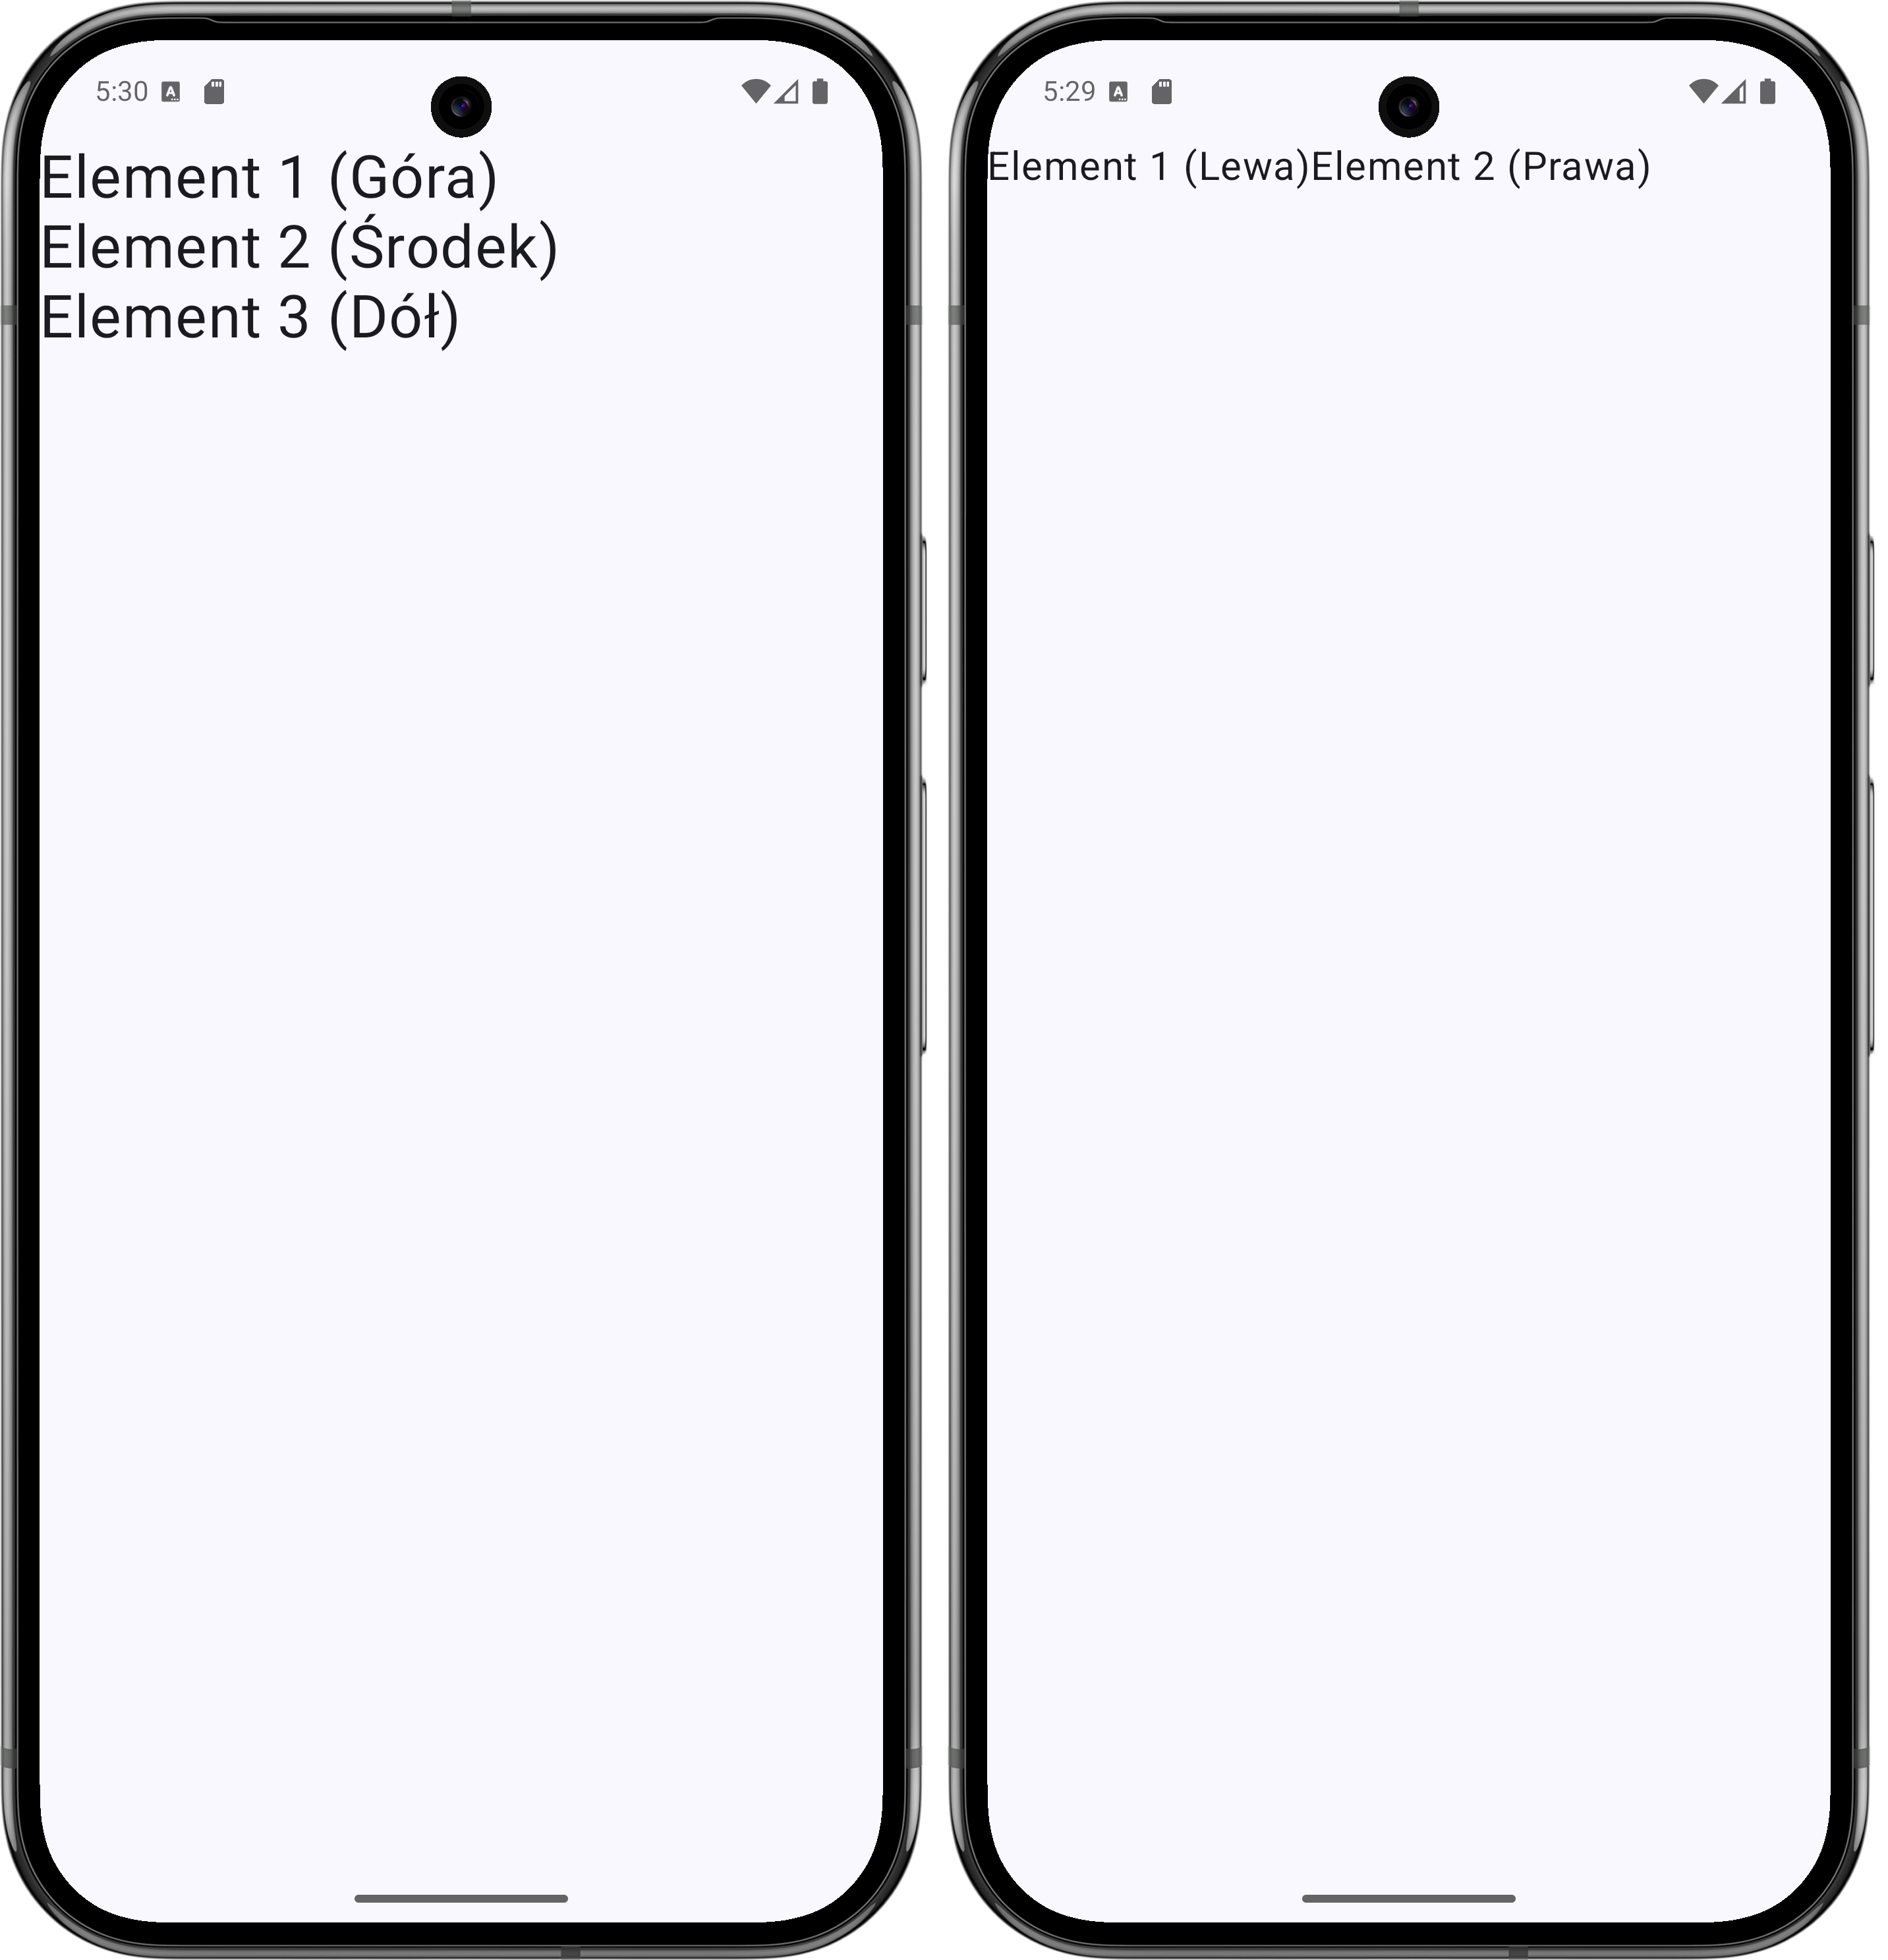
\includegraphics[width=0.4\textwidth]{fig/pum1-w09-column_row_example.png}
    \caption{Przykładowy layout z komponentem \texttt{Column} i \texttt{Row}}
    \label{fig:column_row_example}
\end{figure}

\texttt{Row} układa elementy w poziomie (jeden obok drugiego). Odpowiednik \texttt{LinearLayout} z orientacją poziomą.

\begin{minted}[frame=single,framesep=10pt]{kotlin}
@Composable
fun RowExample() {
    Row {
        Text("Lewa")
        Text("Prawa")
    }
}
\end{minted}

\texttt{Box} układa elementy jeden na drugim (warstwowo). Odpowiednik \texttt{FrameLayout}. Pierwszy element w kodzie ląduje na samym spodzie, a kolejne są rysowane na nim.

\begin{minted}[frame=single,framesep=10pt]{kotlin}
@Composable
fun BoxExample() {
    Box {
        Text("Tło (Pod spodem)")
        Text("Napis (Na wierzchu)")
    }
}
\end{minted}

Siłą Compose jest łatwość łączenia tych komponentów. Poniżej przykład prostego layoutu, gdzie elementy zewnętrzne są ułożone w poziomie, a elementy wewnętrzne w pionie.

\begin{minted}[frame=single,framesep=10pt]{kotlin}
@Composable
fun UserProfile(name: String) {
    Row {
        // Tekst po lewej
        Text(text = "A") 
        
        // Tekst po prawej, ułożony pionowo
        Column {
            Text("Witaj,")
            Text(name)
        }
    }
}
\end{minted}

Do wyświetlania tekstu służy komponent \texttt{Text}. Przy określaniu rozmiarów w Androidzie używamy dwóch jednostek:

\begin{itemize}
    \item \textbf{dp (density-independent pixels)}: Używane do wymiarów (marginesy, szerokość, wysokość). Zapewniają ten sam fizyczny rozmiar elementu na ekranach o różnej gęstości pikseli.
    \item \textbf{sp (scale-independent pixels)}: Używane \textbf{tylko do rozmiaru czcionki}. Działają jak \texttt{dp}, ale dodatkowo uwzględniają ustawienia systemowe użytkownika (np. powiększony tekst dla osób słabowidzących).
\end{itemize}

\section{Modyfikatory (Modifiers)}

\texttt{Modifier} to potężne narzędzie w Compose, które pozwala modyfikować wygląd i zachowanie komponentu (np. dodać tło, margines, obsługę kliknięcia).

Kluczową zasadą jest to, że modyfikatory działają \textbf{sekwencyjnie} (jak łańcuch). Kolejność wywołań ma znaczenie!

\begin{minted}[frame=single,framesep=10pt]{kotlin}
// Przykład: Kolejność paddingu i tła
Box(
    modifier = Modifier
        .background(Color.Red)   // 1. Najpierw czerwone tło
        .padding(16.dp)          // 2. Potem wcięcie (padding) wewnątrz czerwonego tła
        .background(Color.Blue)  // 3. Niebieskie tło wewnątrz paddingu
) {
    Text("Hej!")
}
\end{minted}

Gdybyśmy zamienili kolejność \texttt{padding} i \texttt{background}, efekt wizualny byłby zupełnie inny.

Najczęstsze modyfikatory:
\begin{itemize}
    \item \texttt{.fillMaxSize()}: Zajmij całą dostępną przestrzeń.
    \item \texttt{.padding()}: Odstęp wewnętrzny.
    \item \texttt{.clickable \{ \}}: Reakcja na dotyk.
\end{itemize}

\section{Układ i Wyrównanie (Alignment vs Arrangement)}

Rozmieszczanie elementów w kontenerach \texttt{Row} i \texttt{Column} opiera się na dwóch kluczowych pojęciach: \textbf{osi głównej} (Main Axis) i \textbf{osi poprzecznej} (Cross Axis).

\begin{itemize}
    \item \textbf{Arrangement (Rozmieszczenie)}: Kontroluje układ elementów wzdłuż \textbf{osi głównej}.
    \item \textbf{Alignment (Wyrównanie)}: Kontroluje układ elementów wzdłuż \textbf{osi poprzecznej}.
\end{itemize}

Oznacza to, że dostępne właściwości zależą od używanego kontenera:

\begin{table}[h]
\centering
\begin{tabular}{|c|c|c|}
\hline
\textbf{Kontener} & \textbf{Oś Główna (Arrangement)} & \textbf{Oś Poprzeczna (Alignment)} \\ \hline
\texttt{Column} & Pionowa (\texttt{verticalArrangement}) & Pozioma (\texttt{horizontalAlignment}) \\ \hline
\texttt{Row} & Pozioma (\texttt{horizontalArrangement}) & Pionowa (\texttt{verticalAlignment}) \\ \hline
\end{tabular}
\caption{Osie w kontenerach Row i Column}
\label{tab:axes}
\end{table}

Parametr \texttt{Arrangement} pozwala na precyzyjne określenie odstępów między elementami (dziećmi). Najpopularniejsze opcje to:

\begin{itemize}
    \item \texttt{Arrangement.Start} (dla Row) / \texttt{Top} (dla Column): Elementy \textit{przyklejone} do początku osi.
    \item \texttt{Arrangement.End} (dla Row) / \texttt{Bottom} (dla Column): Elementy \textit{przyklejone} do końca osi.
    \item \texttt{Arrangement.Center}: Elementy zgrupowane na środku osi, stykające się ze sobą.
    \item \texttt{Arrangement.SpaceBetween}: Pierwszy i ostatni element są przy krawędziach, a pozostała przestrzeń jest \textbf{równo} rozdzielona między nimi.
    \item \texttt{Arrangement.SpaceAround}: Podobnie jak SpaceBetween, ale dodaje odstęp również przed pierwszym i po ostatnim elemencie (połowa odstępu wewnętrznego).
    \item \texttt{Arrangement.SpaceEvenly}: Wszystkie odstępy (również te skrajne) są identycznej wielkości.
\end{itemize}

\begin{figure}[h]
    \centering
    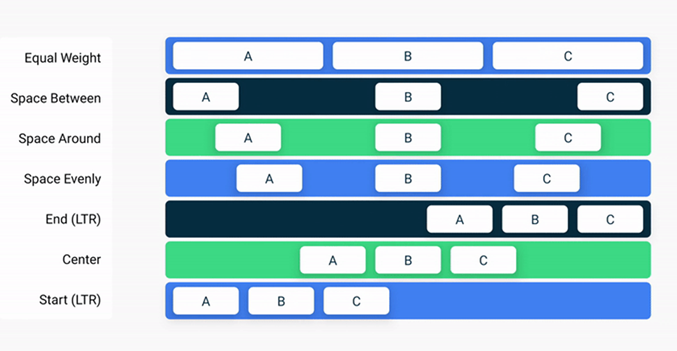
\includegraphics[width=0.8\textwidth]{fig/pum1-w09-arrangement.png}
    \caption{Wizualizacja opcji Arrangement: SpaceBetween, SpaceAround, SpaceEvenly}
    \label{fig:arrangement_viz}
\end{figure}

Czasami zamiast odstępów chcemy, aby element zajmował \textbf{proporcjonalną} część dostępnego miejsca. Służy do tego modyfikator \texttt{weight}.
Jeśli w \texttt{Row} mamy dwa elementy, oba z \texttt{.weight(1f)}, to podzielą one szerokość po równo (50\% / 50\%). Jeżeli chcemy zmienić proporcje, dostosowujemy wagi elementów.

\begin{minted}[frame=single,framesep=10pt]{kotlin}
Row(modifier = Modifier.fillMaxWidth()) {
    // Lewy element zajmie 1/3 (1f / (1f+2f))
    Box(Modifier.weight(1f).background(Color.Red))
    // Prawy element zajmie 2/3 (2f / (1f+2f))
    Box(Modifier.weight(2f).background(Color.Blue))
}
\end{minted}

Poniższy kod centruje element zarówno w pionie, jak i w poziomie. Zauważ, że nazwy parametrów są precyzyjne (\texttt{verticalArrangement} vs \texttt{horizontalAlignment}), co zapobiega pomyłkom.

\begin{minted}[frame=single,framesep=10pt]{kotlin}
Column(
    modifier = Modifier.fillMaxSize(),
    // Oś główna Column = Pionowa -> Arrangement
    verticalArrangement = Arrangement.Center, 
    // Oś poprzeczna Column = Pozioma -> Alignment
    horizontalAlignment = Alignment.CenterHorizontally 
) {
    Text("Na samym środku ekranu")
}
\end{minted}

\begin{figure}[h]
    \centering
    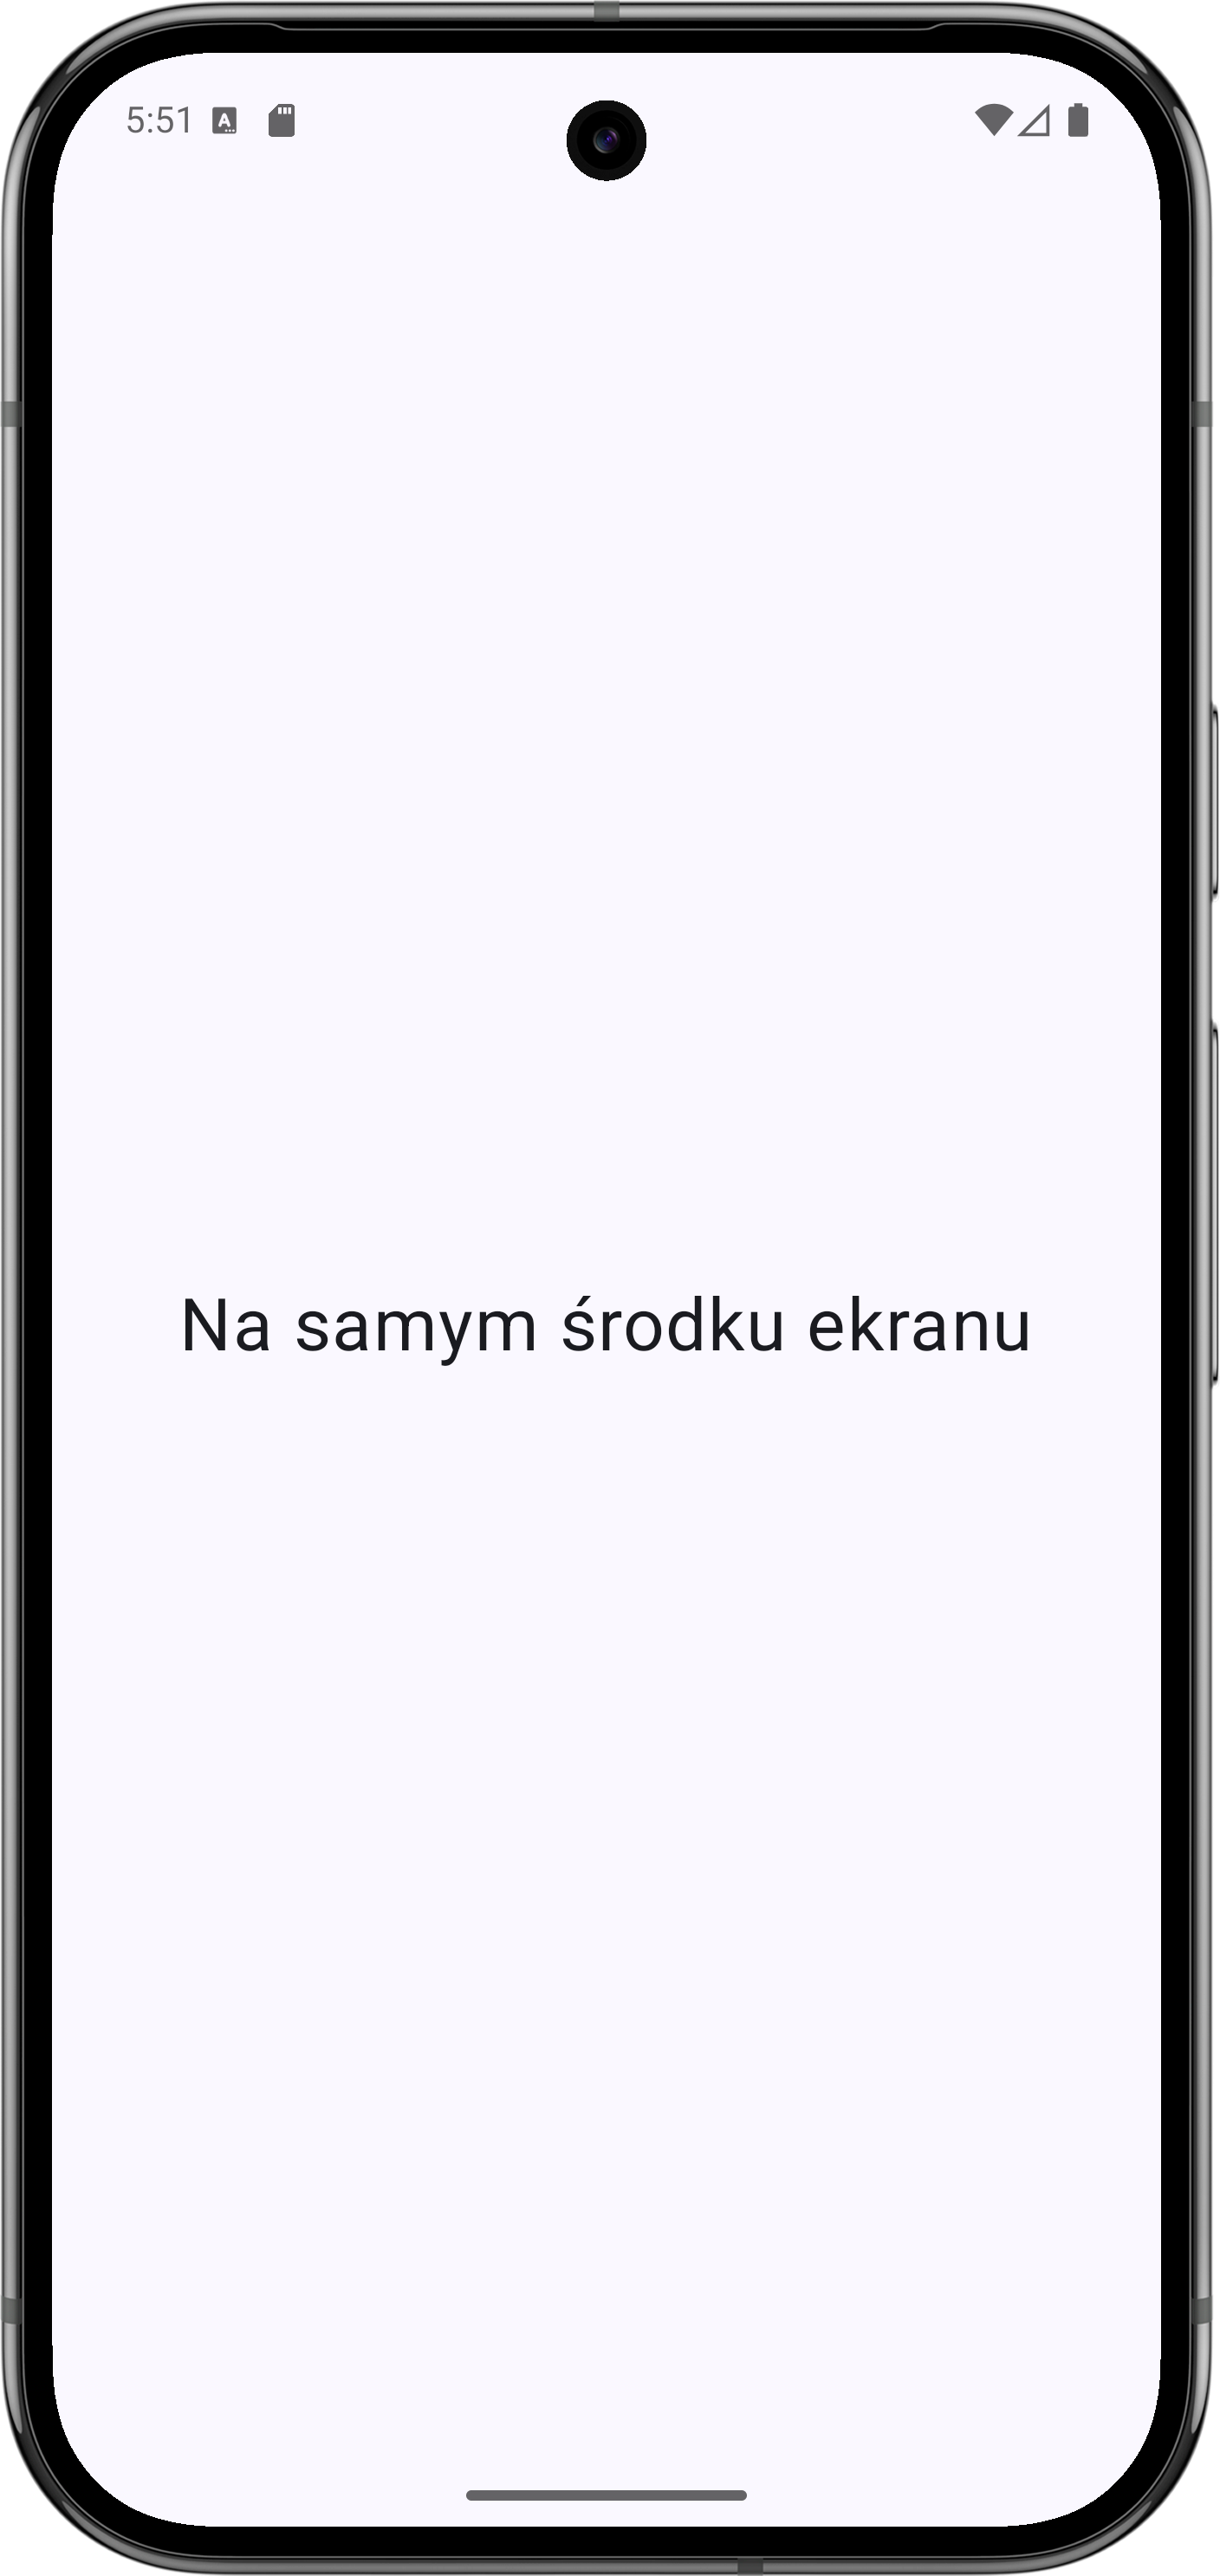
\includegraphics[width=0.25\textwidth]{fig/pum1-w09-arrangement_alignment.png}
    \caption{Wyśrodkowanie elementu w kontenerze}
    \label{fig:arrangement_alignment_viz}
\end{figure}

\section{Zarządzanie Stanem (State)}

Najtrudniejszą zmianą mentalną w Compose jest zrozumienie, czym jest stan i jak wpływa on na UI.

Wyobraź sobie, że interfejs użytkownika (UI) to \textbf{odbicie w lustrze}.
Jeśli jesteś niezadowolony z tego, co widzisz w lustrze (np. masz potargane włosy), nie próbujesz naprawiać samego lustra ani malować po jego powierzchni. Aby zmienić odbicie, musisz zmienić \textbf{obiekt stojący przed lustrem} (czyli uczesać włosy).

W tej analogii:
\begin{enumerate}
    \item \textbf{Lustro} to Framework (Compose). Jest ono nienaruszalne.
    \item \textbf{Odbicie} to Twój Ekran (UI). Jest tylko skutkiem, a nie przyczyną.
    \item \textbf{Obiekt przed lustrem} to \textbf{Stan} (Dane). To tutaj zachodzą zmiany.
\end{enumerate}

Równanie $UI = f(state)$ oznacza, że interfejs jest tylko i wyłącznie wizualną reprezentacją aktualnych danych. Nie można \textit{zmienić tekstu} na ekranie bezpośrednio; można jedynie zmienić zmienną (stan), a Compose (lustro) automatycznie zaktualizuje to, co widzi użytkownik.

W tym miejscu wprowadźmy pojęcia kompozycji i rekompozycji.
\begin{itemize}
    \item \textbf{Kompozycja (Composition)}: To proces, w którym Compose wykonuje Twoje funkcje \texttt{@Composable}, aby zbudować w pamięci opis (drzewo) interfejsu. To definicja UI nakarmiona aktualnymi danymi. Nie jest to jeszcze samo \textit{rysowanie} pikseli, a raczej tworzenie planu tego, co ma zostać narysowane.
    \item \textbf{Rekompozycja (Recomposition)}: To aktualizacja tego opisu. Gdy zmieniają się dane (stan), Compose wykonuje ponownie tylko niezbędne funkcje, aby dostosować drzewo UI do nowej rzeczywistości.
\end{itemize}

Jeśli zmieni się tylko jedna mała liczba w stanie, Compose nie przerysuje całego ekranu. Uruchomi ponownie (zrekomponuje) tylko te funkcje, które korzystają z tej konkretnej liczby. Reszta pozostanie nienaruszona.

\section{Anatomia Funkcji @Composable}

Skoro kompozycja to proces wykonywania funkcji \texttt{@Composable}, musimy zrozumieć, czym one właściwie są. Adnotacja \texttt{@Composable} zmienia typ funkcji w oczach kompilatora.

\begin{itemize}
    \item \textbf{Emisja UI, nie zwracanie wartosci}: Funkcje te zazwyczaj zwracają \texttt{Unit}. Ich celem nie jest zwrócenie obiektu widoku, ale \textbf{wyemitowanie} opisu interfejsu do drzewa kompozycji.
    \item \textbf{Kontekst wywołania}: Funkcję \texttt{@Composable} można wywołać \textbf{tylko} z innej funkcji \texttt{@Composable}. Tworzy to hierarchię wywołań, która startuje od metody \texttt{setContent} w Activity.
    \item \textbf{Zawartość}: Wewnątrz funkcji kompozycyjnej możemy:
    \begin{enumerate}
        \item Wywoływać inne funkcje \texttt{@Composable} (np. \texttt{Text}, \texttt{Column}).
        \item Używać standardowej logiki Kotlina (\texttt{if}, \texttt{for}, \texttt{when}) do sterowania tym, co zostanie wyemitowane.
        \item Zarządzać stanem (\texttt{remember}).
    \end{enumerate}
\end{itemize}

\begin{minted}[frame=single,framesep=10pt]{kotlin}
// Zwykła funkcja - zwraca String
fun formatName(name: String): String {
    return name.uppercase()
}

// Funkcja Composable - emituje UI
@Composable
fun Greeting(name: String) {
    // Możemy używać logiki
    if (name.isNotEmpty()) {
        // I wywoływać inne funkcje Composable
        Text("Witaj, ${formatName(name)}")
    }
}
\end{minted}

\section{Przechowywanie Stanu}

Funkcje w Kotlinie są z natury bezstanowe – gdy funkcja się kończy, jej zmienne lokalne znikają. Jak więc zachować np. stan licznika między odświeżeniami ekranu?

\begin{minted}[frame=single,framesep=10pt]{kotlin}
@Composable
fun Counter() {
    // 1. mutableStateOf tworzy obserwowalny stan (startujemy od 0)
    // 2. remember sprawia, że ta zmienna "przeżyje" rekompozycję
    var count by remember { mutableStateOf(0) }

    Button(onClick = { count++ }) { // Zmiana stanu wyzwala rekompozycję
        // Podczas rekompozycji, Compose widzi nową wartość count
        Text("Kliknięto $count razy") 
    }
}
\end{minted}

Tutaj wchodzą dwaj gracze:

\begin{enumerate}
    \item \texttt{mutableStateOf(value)}: To specjalne \textit{pudełko} na dane, które jest \textbf{obserwowalne}. Gdy zmienisz zawartość tego pudełka (np. \texttt{count.value++}), Compose dostaje sygnał: \textit{"Musisz odświeżyć wszystkich, którzy na to patrzą"}.
    \item \texttt{remember \{ ... \}}: To instrukcja dla kompilatora: \textit{Zapisz ten obiekt w pamięci podręcznej obok drzewa UI}. Gdy funkcja \texttt{Counter} zostanie wywołana ponownie (rekompozycja), \texttt{remember} odda nam zachowaną wcześniej wartość, zamiast tworzyć nową (zresetowaną do zera).
\end{enumerate}

Bez \texttt{remember}, przy każdym kliknięciu funkcja \texttt{Counter} startowałaby od nowa z wartością 0. Bez \texttt{mutableStateOf}, zmiana zmiennej nie dałaby sygnału do odświeżenia ekranu (interfejs byłby martwy).

Mimo że \texttt{remember} działa podczas rekompozycji, ma jedną wadę: \textbf{zapomina wszystko przy zmianie konfiguracji} (np. obrót ekranu, zmiana języka, tryb ciemny). Wtedy cała aktywność jest niszczona i tworzona od nowa, a pamięć podręczna \texttt{remember} jest czyszczona.

Aby zachować stan nawet po \textit{śmierci} i odrodzeniu się aktywności (lub procesu), używamy \texttt{rememberSaveable}. Pod maską wykorzystuje on mechanizm \texttt{Bundle} (ten sam co w \texttt{onSaveInstanceState} z klasycznego Androida).

\begin{minted}[frame=single,framesep=10pt]{kotlin}
@Composable
fun ResilientCounter() {
    // rememberSaveable przeżyje obrót ekranu!
    var count by rememberSaveable { mutableStateOf(0) }

    Button(onClick = { count++ }) {
        Text("Kliknięto $count razy")
    }
}
\end{minted}

Dla prostych typów (Int, String, Boolean) działa to automatycznie. Dla własnych obiektów musimy dostarczyć tzw. \texttt{Saver} (np. implementując \texttt{Parcelable} i używając \texttt{@Parcelize}).

\subsection{Składnia: = vs by}
Często spotkamy się z dwoma zapisami stanu:

\begin{minted}[frame=single,framesep=10pt]{kotlin}
// 1. Przypisanie (=)
val nameState = remember { mutableStateOf("Jan") }
Text(text = nameState.value) // Musimy pisać .value

// 2. Delegacja (by)
var name by remember { mutableStateOf("Jan") }
Text(text = name) // Używamy jak zwykłej zmiennej
\end{minted}

Słowo kluczowe \texttt{by} (delegacja właściwości) \textit{odpakowuje} dla nas stan.
\begin{itemize}
    \item Przy \texttt{by}, zmienna \texttt{name} jest typu \texttt{String} (kompilator ukrywa \texttt{State} pod spodem). Aby zmienić wartość, piszemy \texttt{name = "Ewa"}.
    \item Przy \texttt{=}, zmienna \texttt{nameState} jest typu \texttt{MutableState<String>}. Aby zmienić wartość, musimy pisać \texttt{nameState.value = "Ewa"}.
\end{itemize}
Używanie \texttt{by} wymaga importów (które czasami nie są dodawane automatycznie przez IDE):
\texttt{import androidx.compose.runtime.getValue}
\texttt{import androidx.compose.runtime.setValue}

\section{Wzorzec State Hoisting}

Aby komponenty były wielokrotnego użytku i łatwe w testowaniu, stosujemy wzorzec \textbf{State Hoisting} (wynoszenie stanu w górę). Polega on na tym, że komponent nie zarządza swoim stanem wewnętrznie, ale otrzymuje go od rodzica.

Cechy komponentu \textbf{Stateless} (bezstanowego):
\begin{enumerate}
    \item Otrzymuje stan przez parametr (np. \texttt{value: String}).
    \item Zgłasza zdarzenia przez lambdę (np. \texttt{onValueChange: (String) -> Unit}).
\end{enumerate}

\begin{minted}[frame=single,framesep=10pt]{kotlin}
// Komponent Stateful (zarządza stanem - trudniejszy do testowania i reużycia)
@Composable
fun HelloScreen() {
    var name by remember { mutableStateOf("") }
    HelloContent(name = name, onNameChange = { name = it })
}

// Komponent Stateless (czysta funkcja UI)
@Composable
fun HelloContent(name: String, onNameChange: (String) -> Unit) {
    Column {
        Text("Cześć $name")
        TextField(
            value = name,
            onValueChange = onNameChange
        )
    }
}
\end{minted}

Dzięki temu \texttt{HelloContent} jest niezależny od tego, skąd pochodzi stan (może to być \texttt{remember}, \texttt{ViewModel}, czy stała z testu).
Wzorzec ten promuje \textbf{Unidirectional Data Flow} (Jednokierunkowy Przepływ Danych):
\begin{itemize}
    \item Dane płyną \textbf{w dół} (od rodzica do dziecka).
    \item Zdarzenia płyną \textbf{w górę} (od dziecka do rodzica).
\end{itemize}

\begin{figure}[h]
    \centering
    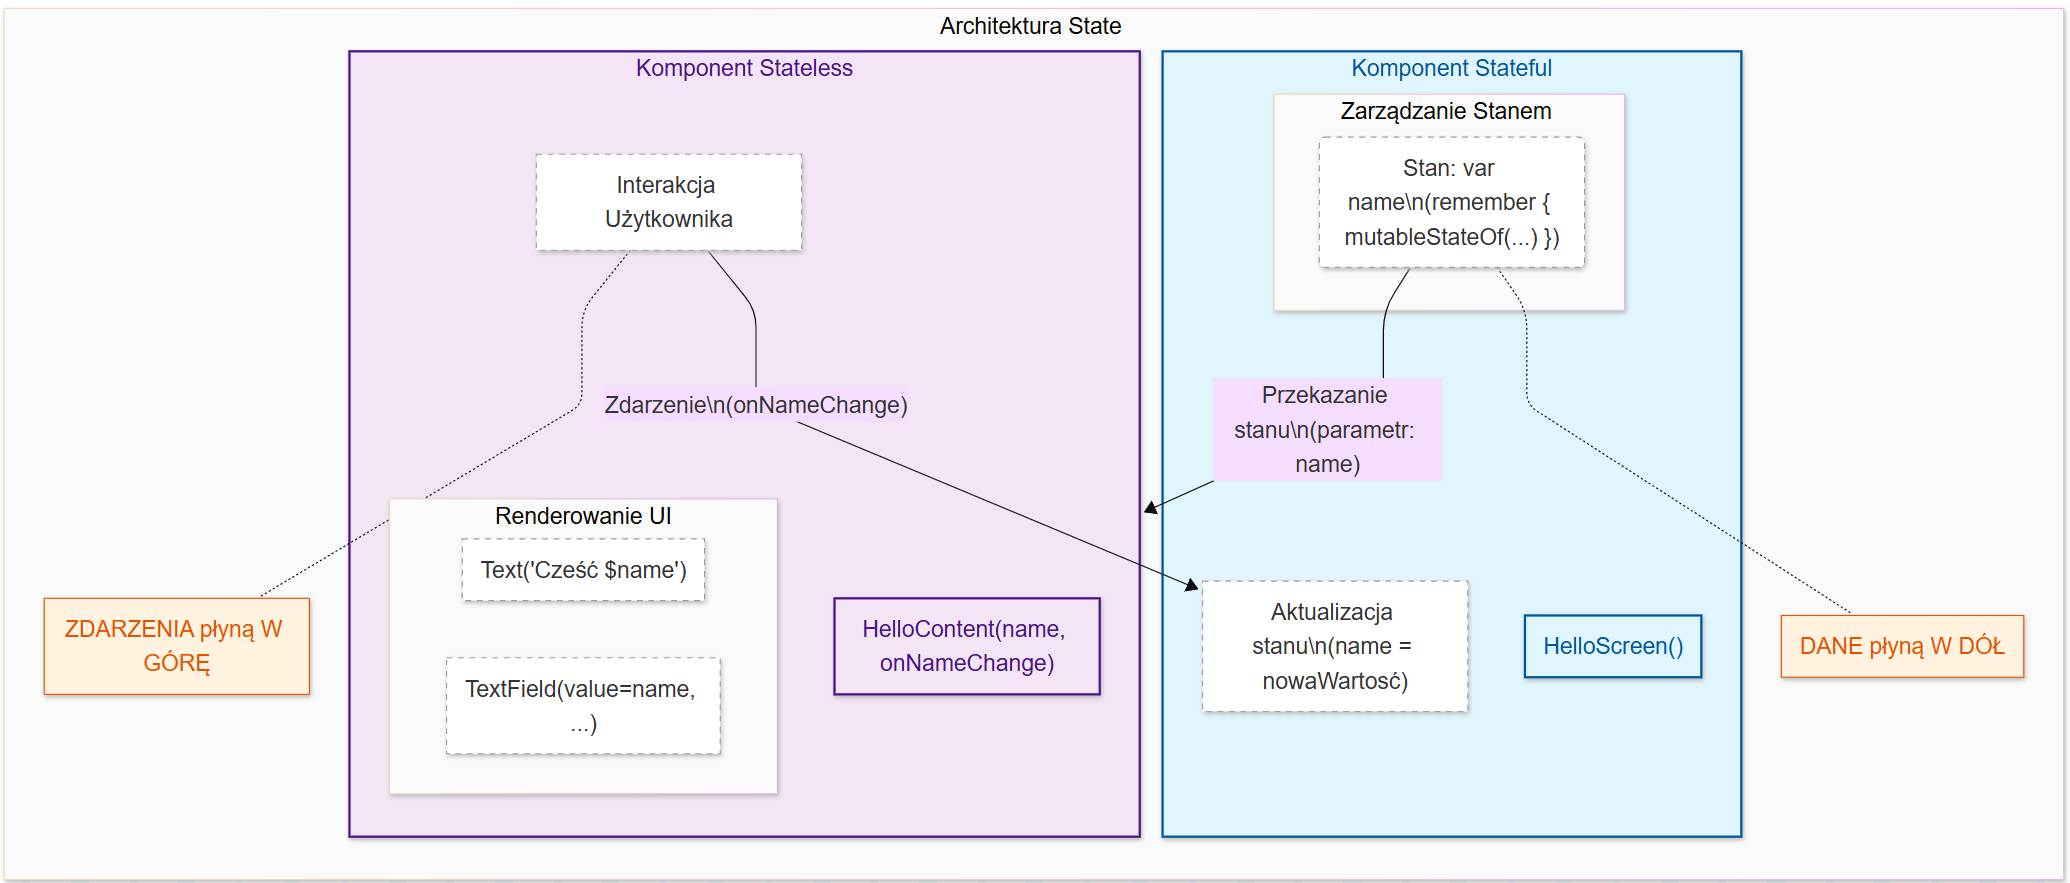
\includegraphics[width=1.0\textwidth]{fig/pum1-w09-state_hoisting.png}
    \caption{Wzorzec State Hoisting}
    \label{fig:pum1-w09-state-hoisting}
\end{figure}
\input{chapters/pum1-w10}
\input{chapters/pum1-w11}
\input{chapters/pum1-w12}
\input{chapters/pum1-w13}
\input{chapters/pum1-w14}

% PUM2
% \part{Programowanie Urządzeń Mobilnych 2}
% \input{chapters/pum2-w01}
% \input{chapters/pum2-w02}
% \chapter{Zaawansowana Współbieżność i pobieranie danych (Wykład 3)}

\section{Ustrukturyzowana Współbieżność}

Poprzednio nauczyliśmy się, jak uruchamiać zadania w tle (\textit{nastawiać wodę}) i nie blokować przy tym kuchni. Co w sytuacji, gdy przygotowanie dania wymaga wykonania \textbf{kilku czynności na raz}, a my musimy mieć pewność, że wszystkie zostały ukończone, zanim wydamy posiłek?

Tu z pomocą przychodzi funkcja \texttt{join()}, która jest fundamentem synchronizacji w świecie korutyn.

Wyobraź sobie, że jesteś Szefem Kuchni (Korutyna-Rodzic). Masz przygotować główne danie: \textit{Stek z warzywami}. Nie będziesz robić wszystkiego sam.
\begin{itemize}
\item Wołasz Pomocnika nr 1: \textit{Usmaż mięso!} (zajmie to 2 sekundy).
\item Wołasz Pomocnika nr 2: \textit{Ugotuj warzywa!} (zajmie to 3 sekundy).
\end{itemize}

Obaj pomocnicy ruszają do pracy w tym samym momencie (współbieżność). Główna korutyn jest wolna i może zająć się innymi sprawami. Ale nie może wydać dania dopóki nie będzie gotowe. To \textit{czekanie} wykonujemy za pomocą \texttt{join()}.

Zobaczmy kod, któy symuluje taką sytuację:

\begin{minted}[frame=single,framesep=10pt]{kotlin}
// 1. Szef Kuchni (Rodzic) rozpoczyna pracę
scope.launch {
    logs.add("Szef kuchni (rodzic): Zaczynamy!")

    // 2. Zlecenie zadania Pomocnikowi 1 (Dziecko 1)
    val jobMieso = launch {
        delay(2000) // Symulacja smażenia
        logs.add("Kucharz 1: Mięso usmażone (2s).")
    }

    // 3. Zlecenie zadania Pomocnikowi 2 (Dziecko 2)
    val jobWarzywa = launch {
        delay(3000) // Symulacja gotowania
        logs.add("Kucharz 2: Warzywa gotowe (3s).")
    }

    logs.add("Szef kuchni: Zadania zlecone, scope czeka na zakończenie...")

    // 4. synchronizacja: Szef czeka na wyniki
    jobWarzywa.join()
    jobMieso.join()

    // 5. Finał
    logs.add("Szef kuchni: Wszyscy skończyli! Można podawać danie.")
}
\end{minted}

W przykładzie widzimy koordynację zadań podrzędnych. Cały proces rozpoczyna się w momencie, gdy korutyna nadrzędna - nasz metaforyczny Szef Kuchni - uruchamia podzadania za pomocą funkcji \texttt{launch}. Jest to swego rodzaju \textit{bilet zamówienia}, który daje nam unikalny uchwyt do konkretnej, trwającej korutyny. W naszym przypadku tworzymy dwa takie uchwyty: \texttt{jobMieso} oraz \texttt{jobWarzywa}, które stają się dziećmi głównej korutyny uruchomionej w scope.

Oba zadania startują niemal w tym samym momencie, co oznacza, że nie czekamy z gotowaniem warzyw do momentu, aż mięso będzie gotowe. Dzięki temu całkowity czas operacji nie jest sumą czasów poszczególnych zadań (5 sekund), lecz odpowiada czasowi najdłuższego z nich (3 sekundy). Jednak ta niezależność podzadań rodzi problem \textbf{synchronizacji}: co, jeśli Szef Kuchni zakończy swoją pracę szybciej niż jego pomocnicy? Bez odpowiedniej kontroli, log \textit{Można podawać danie} pojawiłby się natychmiast po zleceniu zadań, co w naszej metaforze oznaczałoby wydanie klientowi pustego talerza, zanim składniki zdążą się ugotować.

Rozwiązaniem problemu wyścigu (race condition) jest funkcja \texttt{join()}. Z technicznego punktu widzenia jest to funkcja zawieszająca (\texttt{suspend function}), która służy do synchronizacji cyklu życia korutyn. Kiedy korutyna nadrzędna (rodzic) napotyka instrukcję \texttt{jobWarzywa.join()}, jej wykonanie zostaje zawieszone. Należy wyraźnie podkreślić różnicę między zawieszeniem a zablokowaniem: wątek obsługujący tę korutynę nie jest blokowany i może w tym czasie wykonywać inne operacje systemowe. Mechanizm \texttt{join} wprowadza korutynę wywołującą w stan oczekiwania, który trwa dopóki obserwowany obiekt \texttt{Job} nie osiągnie stanu końcowego (Completed lub Cancelled). Dopiero gdy podzadanie faktycznie zakończy swoje działanie, maszyna stanów wznawia korutynę rodzica od kolejnej linii kodu. Dzięki jawnemu wywołaniu \texttt{join()} na obu obiektach \texttt{Job}, realizujemy kontrakt Ustrukturyzowanej Współbieżności, w którym rodzic świadomie koordynuje pracę swoich dzieci i gwarantuje, że żadna operacja nie zostanie zakończona przedwcześnie, zapewniając spójność danych i przewidywalność przepływu aplikacji.

Warto zatrzymać się przy aspekcie, który czyni ustrukturyzowaną współbieżność \textit{bezpieczną} - jest to \textbf{automatyczna propagacja anulowania} - wpominaliśmy już o tym wcześniej. Ale omówmy to jeszcze raz.

Wyobraźmy sobie, że nasz Szef Kuchni (rodzic) otrzymuje informację, że klient anulował zamówienie i wychodzi z restauracji. W świecie \textbf{ustrukturyzowanej współbieżności} Szef nie musi biegać po kuchni i osobiście prosić każdego pomocnika o przerwanie pracy. Wywołanie \texttt{job.cancel()} na korutynie-rodzicu \textbf{automatycznie} przesyła sygnał anulowania do wszystkich dzieci (\texttt{jobMieso}, \texttt{jobWarzywa}). Jeśli pomocnicy wykonują funkcje zawieszające (takie jak \texttt{delay}), natychmiast przerwą pracę.

W programowaniu aplikacji na Androida ten mechanizm jest niezwykle istotny. Kiedy użytkownik zamyka ekran (\texttt{Activity}), powiązany z nim zakres (\texttt{viewModelScope} lub \texttt{lifecycleScope}) zostaje anulowany. Dzięki hierarchii rodzic-dziecko, wszystkie trwające zapytania sieciowe czy obliczenia w tle zostają \textit{posprzątane} automatycznie. Zapobiega to wyciekom pamięci i marnowaniu baterii na procesy, których wyniku nikt już nie zobaczy.

\section{Odbieranie Wyników: Mechanizm \texttt{async} i \texttt{await}}

Mimo że funkcja \texttt{launch} jest niezwykle przydatna, posiada jedno istotne ograniczenie: działa na zasadzie \textit{odpal i zapomnij} (\textit{fire-and-forget}). Zwraca ona obiekt \texttt{Job}, który pozwala nam sprawdzić czy praca trwa, lub ją przerwać, ale nie pozwala nam \textit{wyjąć} ze środka żadnej wartości. W świecie rzeczywistym nie zawsze chcemy tylko zlecić zadanie; często potrzebujemy, aby pracownik coś nam przyniósł (np. konkretny składnik z magazynu). Do takich zadań służy funkcja \texttt{async}.

\subsection{Analogia: Kurier i Pusta Skrzynka} 
Zanim przeanalizujemy kod, posłużmy się analogią zamówienia przesyłki: 
\begin{itemize} 
    \item \textbf{async:} To moment kliknięcia \textit{Kup teraz}. Sklep nie daje nam towaru natychmiast, ale daje nam \textbf{numer śledzenia przesyłki} (to jest nasz obiekt \texttt{Deferred}). 
    \item \textbf{Deferred:} To metaforyczne \textit{puste pudełko}. Pudełko istnieje fizycznie (mamy do niego referencję w kodzie), ale w tej chwili nie możemy z niego skorzystać, bo zawartość jest jeszcze w drodze. 
    \item \textbf{await():} To moment, w którym czekamy na dzwonek kuriera. Jeśli kurier już był - odbieramy zawartość natychmiast. Jeśli jeszcze jedzie - zawieszamy nasze inne czynności i czekamy, aż pudełko zostanie \textit{odpakowane}. 
\end{itemize}

\subsection{Przykład Praktyczny: Generator Tajemniczego Hasła} 
Rozważmy implementację ekranu, który symuluje złożony proces generowania bezpiecznego hasła. Proces ten trwa 3 sekundy i musi zwrócić wynik bezpośrednio do zmiennej stanu interfejsu.

\begin{minted}[frame=single,framesep=10pt]{kotlin}
@Composable fun PasswordGeneratorScreen() { 
    var password by remember { mutableStateOf("...") } 
    val scope = rememberCoroutineScope()

    // Funkcja symulująca ciężkie obliczenia w tle
    suspend fun generatePassword(): String {
        delay(3000) // Symulacja pracy
        return "Kotlin-Is-Super-Secure-123"
    }

    Column(
        modifier = Modifier.fillMaxSize().padding(16.dp),
        horizontalAlignment = Alignment.CenterHorizontally,
        verticalArrangement = Arrangement.Center
    ) {
        Text("Generator Tajemniczego Hasła", style = MaterialTheme.typography.headlineSmall)
        Spacer(Modifier.height(20.dp))

        Button(onClick = {
            password = "Generowanie..."
            
            // Uruchamiamy korutynę nadrzędną (szkielet operacji)
            scope.launch {
                // 1. Zlecenie zadania (async) - natychmiast dostajemy 'pudełko' Deferred
                val deferredPassword: Deferred<String> = async { generatePassword() }
                
                // 2. Oczekiwanie (await) - korutyna zawiesza się tutaj na 3 sekundy
                val result = deferredPassword.await()
                
                // 3. Po 3 sekundach korutyna wznawia pracę z gotowym wynikiem
                password = result
            }
        }) {
            Text("Wygeneruj hasło")
        }

        Spacer(Modifier.height(20.dp))
        Text(password, fontSize = 20.sp, fontFamily = FontFamily.Monospace)
    }
} 
\end{minted}

W powyższym kodzie kluczowy jest moment kliknięcia przycisku. Wywołujemy \path{scope.launch}, aby wejść do świata współbieżności. Wewnątrz niego dzieją się dwie rzeczy: Po pierwsze, linia \texttt{async { generatePassword() }} nie blokuje wykonania kodu. Funkcja \texttt{async} natychmiast zwraca obiekt typu \texttt{Deferred<String>}. Gdybyśmy w tym momencie sprawdzili wartość \texttt{deferredPassword}, dowiedzielibyśmy się jedynie, że zadanie jest w toku. Po drugie, wywołanie \texttt{deferredPassword.await()} jest instrukcją dla mechanizmu korutyn: \textit{Zatrzymaj tę konkretną korutynę w tym miejscu i czekaj, aż} \texttt{deferredPassword} \textit{dostarczy wartość}. Co niezwykle ważne - \textbf{wątek UI pozostaje wolny}. Użytkownik widzi napis \texttt{Generowanie...}, ale aplikacja nie jest zamrożona; system może w tym czasie obsłużyć inne zdarzenia.

Gdy funkcja \texttt{generatePassword()} skończy pracę i zwróci \texttt{String}, \texttt{await()} \textit{odpakuje} go i przypisuje do zmiennej \texttt{result}. Dopiero wtedy wykonuje się ostatnia linia: \texttt{password = result}, co powoduje rekompozycję interfejsu i wyświetlenie hasła.

\section{Most między światami: runBlocking}

Wszystkie funkcje, które poznaliśmy do tej pory - \texttt{launch} oraz \texttt{async} - wymagają do działania istniejącego zakresu (\texttt{CoroutineScope}). Istnieją jednak sytuacje, w których musimy poczekać, aż świat korutyn zakończy swoją pracę, zanim pozwolimy światu zewnętrznemu (blokującemu) ruszyć z miejsca. Do tego celu służy \texttt{runBlocking}. Jak sama nazwa wskazuje, jest to funkcja, która \textbf{blokuje bieżący wątek}, na którym została wywołana, dopóki wszystkie korutyny wewnątrz jej bloku nie zostaną zakończone.

Wyobraź sobie strumień kodu asynchronicznego jako płynącą rzekę - korutyny płyną swobodnie, nie przeszkadzając sobie nawzajem. \texttt{runBlocking} jest jak \textbf{tama}, którą stawiamy w poprzek rzeki. 
\begin{itemize} 
    \item Woda (wątek) przestaje płynąć dalej za tamę. 
    \item Cały nurt zostaje zatrzymany tak długo, aż praca wewnątrz tamy nie zostanie ukończona. 
    \item Dopiero gdy ostatnia korutyna w bloku \texttt{runBlocking} skończy działanie, tama zostaje otwarta i wątek może kontynuować wykonywanie kolejnych linii kodu pod blokiem. 
\end{itemize}

\subsection{Zastosowanie} 
Ponieważ \texttt{runBlocking} blokuje wątek, wywołanie go na wątku UI spowoduje natychmiastowe zamrożenie interfejsu użytkownika na cały czas trwania operacji wewnątrz bloku. Jest to powrót do problemu, który korutyny miały rozwiązać.

Kiedy zatem jest to przydatne? 
\begin{enumerate} 
    \item \textbf{Testy jednostkowe:} W testach chcemy, aby proces testowy poczekał na wynik operacji asynchronicznej, zanim sprawdzi poprawność wyniku (asercję). 
    \item \textbf{Funkcja main():} W prostych programach konsolowych Kotlin, gdzie musimy \textit{zatrzymać} program przed zamknięciem, dopóki korutyny nie skończą pracy. 
    \item \textbf{Integracja z kodem blokującym:} Gdy musimy wywołać kod asynchroniczny wewnątrz biblioteki, która nie wspiera korutyn i wymaga natychmiastowego zwrotu wartości. 
\end{enumerate}

\subsection{Porównanie mechanizmów} 
Poniższy przykład pokazuje, jak \texttt{runBlocking} wpływa na przepływ programu w porównaniu do \texttt{launch}.

\begin{minted}[frame=single,framesep=10pt]{kotlin} 
fun runBlockingExample() { 
    println("1. Start programu")

    // Ten blok zatrzyma wątek na 2 sekundy!
    runBlocking {
        println("2. Wewnątrz runBlocking - start")
        delay(2000)
        println("3. Wewnątrz runBlocking - koniec")
    }

    println("4. Koniec programu - ta linia czekała na tamę")
} 
\end{minted}

W powyższym kodzie napis \textit{4. Koniec programu} pojawi się dopiero po 2 sekundach. Gdybyśmy zamiast \texttt{runBlocking} użyli \texttt{launch} (w odpowiednim \texttt{scope}), napis \textit{4} pojawiłby się natychmiast po napisie \textit{2}, ponieważ rzeka płynęłaby dalej, podczas gdy korutyna pracowałaby \textit{obok}.
% \chapter{Podstawy Architektury Aplikacji (Wykład 4)}

\section{Problem Monolitycznego Kodu ("God Composable")}

Na początku przygody z Jetpack Compose naturalnym odruchem jest pisanie całego kodu wewnątrz funkcji \texttt{@Composable}. Skoro UI to tylko funkcja, dlaczego nie umieścić w niej również pobierania danych z sieci czy logiki biznesowej?

Spójrzmy na kod, który działa, ale łamie zasady inżynierii oprogramowania. Nazywamy to antywzorcem \textbf{"God Composable"} - funkcją, która wie i robi wszystko.

\begin{minted}[frame=single,framesep=10pt]{kotlin}
// KROK 1: Kod "naiwny"
@Composable
fun UserProfileScreen() {
    // Stan UI + Logika w jednym miejscu
    var userData by remember { mutableStateOf("Ładowanie...") }
    val scope = rememberCoroutineScope() // Scope powiązany z cyklem życia UI

    Column {
        Button(onClick = {
            // Operacja sieciowa bezpośrednio w UI
            scope.launch {
                try {
                    val user = api.getUser() // Symulacja pobierania (2 sekundy)
                    userData = user.name.uppercase() // Logika biznesowa
                } catch (e: Exception) {
                    userData = "Błąd!"
                }
            }
        }) {
            Text("Pobierz dane")
        }
        Text(userData)
    }
}
\end{minted}

\subsection{Rotacja Ekranu}
Uruchamiamy aplikację, klikamy przycisk, dane się pobierają. Wszystko wygląda świetnie. Do momentu, gdy obrócimy telefon.
Android przy zmianie konfiguracji (np. obrót ekranu) niszczy i tworzy aktywność od nowa. Funkcja \texttt{remember} traci pamięć. Użytkownik, który czekał na dane, nagle znów widzi ekran początkowy \texttt{Ładowanie...}.

\subsection{Próba ratunku: rememberSaveable}
Rozwiązanie tego problemu już znamy z poprzedniego semestru. Spróbujmy więc naprawić nasz kod:

\begin{minted}[frame=single,framesep=10pt]{kotlin}
// rememberSaveable
var userData by rememberSaveable { mutableStateOf("Ładowanie...") }
\end{minted}

Czy to rozwiązuje problem? Tylko pozornie i tylko w trywialnych przypadkach. Gdy spróbujemy zastosować to w większej aplikacji, napotkamy trzy krytyczne problemy, których \texttt{rememberSaveable} nie rozwiąże:

\begin{itemize}
    \item \textbf{Śmierć Korutyny:} \texttt{rememberCoroutineScope} jest ściśle powiązany z widokiem. Gdy obracasz ekran w trakcie pobierania danych (np. wolne WiFi), stary widok ginie, a wraz z nim \textbf{anulowana jest korutyna}. Pobieranie zostaje przerwane w połowie. Nowy ekran powstaje, ale nic nie wie o tym, że poprzedni coś pobierał. Użytkownik klika, czeka i nic nie dostaje.
    
    \item \textbf{Ograniczenia Pamięci (Bundle):} \texttt{rememberSaveable} zapisuje dane w systemowym \texttt{Bundle}. Jest on przeznaczony dla małych danych (tekst, liczby). Jeśli spróbojemy tam zapisać listę 500 obiektów JSON pobranych z API, aplikacja wyrzuci błąd \texttt{TransactionTooLargeException} i się zamknie.
    
    \item \textbf{Testowalność:} Jak przetestować, czy nazwisko jest poprawnie zamieniane na wielkie litery? W obecnym kodzie jest to niemożliwe bez uruchamiania emulatora, bo logika jest \textit{zabetonowana} wewnątrz przycisku.
\end{itemize}

\subsection{Separacja odpowiedzialności}
Dochodzimy do wniosku, że funkcja \texttt{Composable} nie jest odpowiednim miejscem na trzymanie danych ani wykonywanie operacji. Potrzebujemy miejsca, które:
\begin{enumerate}
    \item Przeżyje rotację ekranu (nie jak \texttt{rememberSaveable}).
    \item Pozwoli korutynom dokończyć pracę, nawet gdy widok jest niszczony.
    \item Nie ma limitu wielkości danych (nie jak \texttt{Bundle}).
\end{enumerate}

\subsection{Metafora Budowlana: Buda vs Wieżowiec}
Aby zrozumieć potrzebę architektury, posłużmy się analogią budowlaną:
\begin{itemize}
    \item \textbf{Budowanie budy dla psa (Brak architektury):} Możesz to zrobić sam. Jeśli wbijesz gwóźdź w złym miejscu, łatwo to poprawić. To są małe, proste aplikacje.
    \item \textbf{Budowanie wieżowca (Z architekturą):} Tutaj potrzebujesz planu. Elektryk (Data Layer) nie maluje ścian, a malarz (UI Layer) nie kładzie instalacji gazowej. W dużym projekcie, jeśli Composable zajmuje się logiką API, to tak jakby malarz próbował naprawiać windę.
\end{itemize}

Potrzebujemy więc "Kierownika Budowy", który ma plany w biurze (bezpiecznym od remontów) i zarządza pracami. Tym kierownikiem będzie komponent, który za chwilę poznamy.

\section{Ewolucja Wzorców Architektonicznych}

Skoro wiemy już, że wrzucanie wszystkiego do jednego worka ("God Composable") jest nie najlepszym rozwiązaniem, musimy zastanowić się, jak podzielić aplikację. W inżynierii oprogramowania ten problem nie jest nowy. Przez dekady wykształciło się wiele różnych podejść do tego problemu. Jednym z nich jest rodzina wzorców MVx, które różnią się sposobem, w jaki warstwa danych komunikuje się z warstwą wizualną.

Aby zrozumieć różnice między nimi, posłużymy się analogiami z życia codziennego.

\subsection{MVC (Model-View-Controller) - Sklep z ladą}


[Image of MVC architecture diagram]

Jest to najstarsze podejście, które można porównać do wizyty w tradycyjnym sklepie, gdzie towar podaje sprzedawca.

\begin{itemize}
    \item \textbf{Ty (View):} Stoisz przed ladą. Widzisz towar, ale jesteś pasywny - nie możesz go sam wziąć.
    \item \textbf{Sprzedawca (Controller):} To on rządzi procesem. Mówisz mu: \textit{Poproszę chleb} (Interakcja).
    \item \textbf{Magazyn (Model):} Sprzedawca idzie na zaplecze, sprawdza stan magazynowy i bierze towar.
\end{itemize}

\textbf{Wniosek:} W tym układzie Sprzedawca (Controller) decyduje o wszystkim. To on musi wiedzieć, jak wygląda magazyn i to on decyduje, co pokazać klientowi. Musi też być w stanie wskazać konkretnego klienta, któremu musi wydać towar.

\subsection{MVP (Model-View-Presenter) - Restauracja}

Druga odmiana wzorca z rodziny MVx.

\begin{itemize}
    \item \textbf{Klient przy stoliku (View):} Siedzisz i czekasz. Nie wiesz i nieinteresuje Cię, co się dzieje w kuchni.
    \item \textbf{Kelner (Presenter):} Przyjmuje zamówienie i idzie do kuchni (Model).
    \item \textbf{Kluczowa cecha:} Kelner wraca z kuchni i \textbf{własnoręcznie stawia talerz na Twoim stole}.
\end{itemize}

W kodzie wygląda to tak, że Presenter (Kelner) posiada referencję do Widoku (Klienta). Wywołuje na nim konkretną metodę, np. \texttt{view.showDinner()}.
\textbf{Problem:} Jest to sztywne połączenie 1:1. Kelner musi znać konkretny stolik. Jeśli Klient wyjdzie do toalety (Rotacja Ekranu/Zniszczenie Widoku), a Kelner wróci z talerzem i spróbuje go postawić na pustym miejscu, dojdzie do błędu (\texttt{NullPointerException}).

\subsection{MVVM (Model-View-ViewModel) - Automat z napojami}

To podejście jest standardem we współczesnym Androidzie i idealnie współgra z Jetpack Compose.

\begin{itemize}
    \item \textbf{Użytkownik (View):} Podchodzi do maszyny i naciska przycisk (Wysyła Event).
    \item \textbf{Automat (ViewModel):} Odbiera sygnał, mieli kawę, pobiera wodę (komunikuje się z Repozytorium/Modelem).
    \item \textbf{Wynik (State):} Automat wystawia kubek z kawą do szuflady odbiorczej (\textit{Emisja stanu}).
\end{itemize}

\textbf{Kluczowa różnica - Reaktywność:} Automatu nie obchodzi, kto ten kubek weźmie.
\begin{itemize}
    \item Automat tylko \textbf{wystawia stan}.
    \item Jeśli nikt nie stoi przed maszyną - kubek (dane) po prostu czeka w szufladzie.
    \item Jeśli użytkownik odejdzie (obróci ekran) i przyjdzie nowy (\texttt{Activity} zostanie stworzone na nowo) - kubek z kawą nadal tam jest. Nowy widok po prostu zagląda do szuflady i widzi gotowy napój.
\end{itemize}

W Compose tą \textit{szufladą} są strumienie danych, takie jak \texttt{StateFlow}. ViewModel aktualizuje \texttt{StateFlow}, a Widok (Composable) jedynie nasłuchuje zmian. To rozwiązuje nasz problem z rotacją ekranu - ViewModel trzyma \textit{napój}, niezależnie od tego, co dzieje się z \textit{klientem}.

\subsection{MVI (Model-View-Intent) - Kiosk samoobsługowy}

Jest to ewolucja wzorca MVVM, która kładzie rygorystyczny nacisk na jednokierunkowy przepływ danych (Unidirectional Data Flow).

\begin{itemize}
    \item \textbf{View (Ekran kiosku):} Wyświetla aktualny stan zamówienia. Jest to \textit{tylko odczyt}.
    \item \textbf{Intent (Zamiar/Akcja):} Gdy klikasz \textit{Dodaj frytki}, nie zmieniasz bezpośrednio zamówienia. Wysyłasz do systemu \textit{zamiar} (Intent) o treści: "Użytkownik chce dodać frytki".
    \item \textbf{Model (System):} System bierze Twój \textit{aktualny paragon}, bierze Twój \textit{zamiar}, przetwarza je i wypluwa \textbf{zupełnie nowy, zaktualizowany paragon} (State).
\end{itemize}

\textbf{Kluczowa cecha - Cykliczność i Niezmienność:}
W przeciwieństwie do MVVM, gdzie ViewModel może mieć wiele różnych strumieni danych (osobno imię, osobno lista, osobno błędy), w MVI dążymy do posiadania \textbf{jednego obiektu stanu} (np. \texttt{OrderUiState}).
W naszej metaforze: Nie możesz wziąć długopisu i dopisać frytek do wydrukowanego paragonu. Musisz wysłać żądanie, a system wydrukuje Ci nowy, zaktualizowany paragon. To zapewnia przewidywalność aplikacji - zawsze wiemy, co doprowadziło do obecnego stanu ekranu.

W Jetpack Compose naturalnie dążymy do MVI, używając pojedynczego \texttt{StateFlow<UiState>} w ViewModelu.
% \input{chapters/pum2-w05}
% \input{chapters/pum2-w06}
% \chapter{Kanały (Channels): Komunikacja i Synchronizacja (Wykład 7)}

W poprzednich rozdziałach do przesyłania danych używaliśmy strumieni (\texttt{Flow}). Strumień działał jak radio: stacja nadawcza emitowała sygnał, a każdy, kto nastroił odbiornik (\texttt{collect}), otrzymywał te same dane.

Co jednak w sytuacji, gdy potrzebujemy precyzyjnej komunikacji \textit{jeden-do-jednego}? Wyobraźmy sobie fabrykę: jedna maszyna produkuje śruby, a druga je pakuje. Każda śruba wyprodukowana przez maszynę A musi trafić do maszyny B. Nie chcemy, aby śruba zaginęła, ani żeby trafiła do dwóch paczek naraz. Do takich zadań Kotlin udostępnia osobny prymityw synchronizacyjny: \textbf{Kanały (Channels)}.

Kanał (\texttt{Channel}) to koncepcyjnie taśmociąg łączący dwie korutyny.
\begin{itemize}
    \item \textbf{Nadawca (Producer):} Wrzuca dane z jednej strony rury.
    \item \textbf{Odbiorca (Consumer):} Wyciąga dane z drugiej strony.
\end{itemize}

\begin{figure}[htbp]
    
\includegraphics[width=0.7\textwidth]{fig/pum2-w07-channel.png}
    \caption{\texttt{Channel}.}
    \label{fig:Figura channel}
\end{figure}

Kluczową cechą kanałów jest to, że służą one nie tylko do przesyłania danych, ale także do \textbf{synchronizacji} pracy korutyn. Jeśli rura jest pusta, odbiorca czeka. Jeśli rura jest pełna (w przypadku kanałów buforowanych), nadawca czeka.

\section{Channel vs Flow (SharedFlow)}

Różnica jest fundamentalna i dotyczy modelu dystrybucji danych.

\begin{table}[h]
\centering
\begin{tabularx}{\linewidth}{|l|X|X|}
\hline
\textbf{Cecha} & \textbf{Flow (SharedFlow)} & \textbf{Channel} \\ \hline

\textbf{Model komunikacji} &
\textbf{Multicast} (Jeden do Wielu) &
\textbf{Unicast} (Jeden do Jednego*) \\ \hline

\textbf{Metafora} &
\textbf{Radio / Telewizja}. Wszyscy subskrybenci słyszą to samo. Jeśli nikt nie słucha, audycja i tak leci (SharedFlow) lub w ogóle nie startuje (Cold Flow). &
\textbf{Poczta / Walkie-Talkie}. List trafia do jednej skrzynki. Jeśli jest dwóch odbiorców, ten szybszy zabierze list, a drugi zobaczy pustą skrzynkę. \\ \hline

\textbf{Dystrybucja elementu} &
Każdy element trafia do \textbf{wszystkich} aktywnych subskrybentów. &
Każdy element trafia tylko do \textbf{jednego} odbiorcy. \\ \hline

\textbf{Zastosowanie} &
Stan UI, aktualizacje bazy danych, zdarzenia globalne. &
Kolejki zadań, przesyłanie wyników między wątkami tła. \\ \hline
\end{tabularx}
\caption{Porównanie Flow i Channel}
\end{table}

% \begin{table}[h]
% \centering
% \begin{tabular}{|l|p{6cm}|p{3cm}|}
% \hline
% \textbf{Cecha} & \textbf{Flow (SharedFlow)} & \textbf{Channel} \\ \hline
% \textbf{Model komunikacji} & \textbf{Multicast} (Jeden do Wielu) & \textbf{Unicast} (Jeden do Jednego*) \\ \hline
% \textbf{Metafora} & \textbf{Radio / Telewizja}. Wszyscy subskrybenci słyszą to samo. Jeśli nikt nie słucha, audycja i tak leci (SharedFlow) lub w ogóle nie startuje (Cold Flow). & \textbf{Poczta / Walkie-Talkie}. List trafia do jednej skrzynki. Jeśli jest dwóch odbiorców, ten szybszy zabierze list, a drugi zobaczy pustą skrzynkę. \\ \hline
% \textbf{Dystrybucja elementu} & Każdy element trafia do \textbf{wszystkich} aktywnych subskrybentów. & Każdy element trafia tylko do \textbf{jednego} odbiorcy. \\ \hline
% \textbf{Zastosowanie} & Stan UI, aktualizacje bazy danych, zdarzenia globalne. & Kolejki zadań, przesyłanie wyników między wątkami tła. \\ \hline
% \end{tabular}
% \caption{Porównanie Flow i Channel}
% \end{table}

\textit{Uwaga: Kanał może mieć wielu odbiorców, ale wtedy działają oni jak konkurencyjni pracownicy - każdy element zostanie obsłużony tylko przez jednego z nich. W SharedFlow każdy pracownik dostałby kopie wszystkich zadań.}

\begin{itemize}
    \item Użyj \textbf{StateFlow/SharedFlow}, gdy dane mają trafić do warstwy UI (Widoku). UI zazwyczaj tylko \textit{obserwuje} stan i nie \textit{konsumuje} go bezpowrotnie.
    \item Użyj \textbf{Channel}, gdy implementujesz mechanizm producent-konsument wewnątrz logiki biznesowej (np. kolejka plików do wysłania na serwer).
\end{itemize}

\section{Podstawowe API: send() i receive()}

W przeciwieństwie do \texttt{Flow}, który definiujemy deklaratywnie, obsługa Kanału przypomina obsługę tradycyjnej kolejki, ale z jedną kluczową różnicą: jest ona \textbf{asynchroniczna}.

Interfejs \texttt{Channel<T>} implementuje dwa mniejsze interfejsy:
\begin{itemize}
    \item \texttt{SendChannel<T>} - pozwala tylko wysyłać i zamykać kanał.
    \item \texttt{ReceiveChannel<T>} - pozwala tylko odbierać dane.
\end{itemize}

Dzięki temu możemy przekazać odbiorcy tylko interfejs \texttt{ReceiveChannel}, mając pewność, że przez pomyłkę nic nie wyśle ani nie zamknie kanału. Dwie główne metody obsługi kanału to \texttt{send(element)} oraz \texttt{receive()}. Obie są funkcjami zawieszającymi (\texttt{suspend}).

\begin{enumerate}
    \item \textbf{receive() zawiesza}, gdy kanał jest \textbf{pusty}.
    Konsument podchodzi do taśmociągu. Jeśli nie ma tam żadnej paczki, nie blokuje wątku (nie stoi bezczynnie). Korutyna zawiesza się (\textit{idzie na przerwę}) i zostanie wznowiona dopiero, gdy Nadawca wrzuci coś do kanału.

    \item \textbf{send() zawiesza}, gdy kanał jest \textbf{pełny}.
    Jeśli taśmociąg ma ograniczoną pojemność (co omówimy w sekcji 7.4) i jest zapchany, Nadawca nie może wrzucić nowej paczki. Korutyna zawiesza się i czeka, aż Konsument zdejmie coś z taśmy, robiąc miejsce.
\end{enumerate}

\begin{minted}[frame=single,framesep=10pt]{kotlin}
val channel = Channel<Int>()

// KORUTYNA 1: Producent
launch {
    for (x in 1..5) {
        // Jeśli odbiorca nie jest gotowy, send() zawiesi tę korutynę
        channel.send(x * x) 
        delay(100)
    }
    // Ważne: Sygnał, że więcej danych nie będzie
    channel.close() 
}

// KORUTYNA 2: Konsument
launch {
    // Pętla for automatycznie kończy działanie, 
    // gdy kanał zostanie zamknięty
    for (y in channel) {
        println("Odebrano: $y")
    }
    println("Kanał zamknięty, koniec pracy.")
}
\end{minted}

Kanał jest koncepcyjnie \textit{otwarty} tak długo, jak go nie zamkniemy. W przeciwieństwie do \texttt{Flow}, który kończy się naturalnie po wykonaniu bloku kodu, Kanał może działać w nieskończoność.

\begin{figure}[htbp]
    \includegraphics[width=1.0\textwidth]{fig/pum2-w07-kanaly.png}
    \caption{Kanały.}
    \label{fig:channels}
\end{figure}

Metoda \texttt{close()} wysyła specjalny sygnał \textit{koniec transmisji}.
\begin{itemize}
    \item Próba wysłania (\texttt{send}) na zamknięty kanał rzuci wyjątek \texttt{ClosedSendChannelException}.
    \item Próba odbioru (\texttt{receive}) z zamkniętego kanału (gdy bufor jest pusty) rzuci wyjątek \texttt{ClosedReceiveChannelException}.
\end{itemize}

Częściej można się spotkać z zastosowaniem \texttt{for (item in channel)}, która automatycznie obsługuje zamknięcie kanału i bezpiecznie wychodzi z pętli.

\section{Rodzaje Kanałów (Buforowanie)}

Konstruktor klasy \texttt{Channel} przyjmuje opcjonalny parametr \texttt{capacity}. To on decyduje o tym, kiedy funkcja \texttt{send()} zawiesi nadawcę. Wybór odpowiedniego typu bufora jest kluczowy dla zarządzania przepływem danych.

\subsection{Rendezvous (Domyślny)}
\texttt{capacity = Channel.RENDEZVOUS} (lub 0).

To domyślny i najbardziej restrykcyjny typ kanału. Nie posiada on żadnego bufora.
\begin{itemize}
    \item \textbf{Działanie:} Nadawca i Odbiorca muszą się \textit{spotkać} (fr. \textit{rendezvous}) w tym samym momencie.
    \item \textbf{Zachowanie:} \texttt{send()} zawiesza się dopóki druga strona nie wywoła \texttt{receive()}. I odwrotnie.
    \item \textbf{Metafora:} Przekazywanie pałeczki w sztafecie. Biegacz A nie może puścić pałeczki, dopóki B jej nie chwyci.
\end{itemize}

Jest to idealne rozwiązanie do ścisłej synchronizacji dwóch wątków.

\subsection{Buffered (Buforowany)}
\texttt{capacity = liczba dodatnia} (np. 10).

Kanał posiada kolejkę o ustalonym rozmiarze (\texttt{ArrayChannel}).
\begin{itemize}
    \item \textbf{Działanie:} Nadawca może wysłać tyle elementów, ile mieści bufor, nie czekając na odbiorcę.
    \item \textbf{Zachowanie:} \texttt{send()} zawiesza się dopiero, gdy bufor jest \textbf{pełny}.
    \item \textbf{Metafora:} Taśmociąg w fabryce. Maszyna produkująca może pracować szybciej przez chwilę, zapełniając taśmę, nawet jeśli maszyna pakująca chwilowo stanęła.
\end{itemize}

\subsection{Conflated (Scalony/Nadpisujący)}
\texttt{capacity = Channel.CONFLATED}.

Specyficzny kanał o pojemności 1, który nigdy nie wstrzymuje nadawcy.
\begin{itemize}
    \item \textbf{Działanie:} Jeśli odbiorca nie nadąża, stare elementy są \textbf{wyrzucane}, a w kanale zostaje tylko ten najnowszy.
    \item \textbf{Zachowanie:} \texttt{send()} \textbf{nigdy} się nie zawiesza.
    \item \textbf{Metafora:} Tablica z kursami walut. Nie interesuje nas historia zmian z ostatnich 5 minut, chcemy widzieć tylko aktualną cenę.
\end{itemize}

\subsection{Unlimited (Nielimitowany)}
\texttt{capacity = Channel.UNLIMITED}.

Kanał z buforem opartym na liście łączonej (\texttt{LinkedList}), która rośnie w \textit{nieskończoność}.

\begin{itemize}
    \item \textbf{Działanie:} Przyjmuje wszystko.
    \item \textbf{Zachowanie:} \texttt{send()} \textbf{nigdy} się nie zawiesza (chyba że braknie pamięci RAM).
    \item \textbf{Ostrzeżenie:} Używanie tego kanału jest ryzykowne. Jeśli nadawca jest szybszy od odbiorcy, program w końcu wyrzuci błąd \texttt{OutOfMemoryError}.
\end{itemize}

\begin{figure}[htbp]
    \includegraphics[width=1.0\textwidth]{fig/pum2-w07-channels_types.png}
    \caption{Rodzaje kanałów.}
    \label{fig:channels_types}
\end{figure}

\subsection{Przykład konfiguracji}

\begin{minted}[frame=single,framesep=10pt]{kotlin}
// 1. Rendezvous (domyślny) - ścisła synchronizacja
val c1 = Channel<Int>() 

// 2. Buffered - bufor na 10 elementów
val c2 = Channel<Int>(10)

// 3. Conflated - tylko najnowsza wartość
val c3 = Channel<Int>(Channel.CONFLATED)
\end{minted}

Warto zauważyć, że \texttt{StateFlow} działa bardzo podobnie do kanału typu \texttt{Conflated} (trzyma tylko najnowszy stan), podczas gdy zwykły \texttt{Flow} z buforem zachowuje się jak kanał \texttt{Buffered}.

\section{Instrukcja select}

W standardowym kodzie asynchronicznym (używając \texttt{await} lub \texttt{receive}) czekamy sekwencyjnie: najpierw na wynik A, potem na wynik B. Mamy jeszcze jedną możliwość: możemy przetworzyć wynik z tego, które odpowie \textbf{szybciej} za pomocą wyrażenia \texttt{select}. Pozwala ono \textit{nasłuchiwać} na wielu kanałach (lub obiektach \texttt{Deferred}) jednocześnie i uruchomić kod skojarzony tylko z tym zdarzeniem, które nastąpi jako pierwsze.

Wyrażenie \texttt{select<T>} zwraca wynik typu \texttt{T}. Wewnątrz bloku definiujemy klauzule (np. \texttt{onReceive}), które mówią \textit{co zrobić, jeśli to źródło wygra wyścig}.

\begin{minted}[frame=single,framesep=10pt]{kotlin}

suspend fun raceData() {
    val server1 = Channel<String>()
    val server2 = Channel<String>()

    // Symulacja: Serwer 1 jest wolny
    launch {
        delay(500)
        server1.send("Dane z USA (500ms)")
    }

    // Symulacja: Serwer 2 jest szybki
    launch {
        delay(100)
        server2.send("Dane z Europy (100ms)")
    }

    // WYŚCIG: Czekamy na PIERWSZY wynik
    val winner = select<String> {
        // Klauzula 1: Jeśli server1 wyśle pierwszy...
        server1.onReceive { msg ->
            "Wygrał Serwer 1: $msg"
        }
        
        // Klauzula 2: Jeśli server2 wyśle pierwszy...
        server2.onReceive { msg ->
            "Wygrał Serwer 2: $msg"
        }
    }

    println(winner)
}
\end{minted}

\subsection{Zastosowanie Praktyczne: Timeout}

Najczęstszym zastosowaniem \texttt{select} jest zastosowanie \texttt{onTimeout}, aby \textbf{zrezygnować z czekania}, jeśli operacja trwa zbyt długo.

\begin{minted}[frame=single,framesep=10pt]{kotlin}
val dataChannel = Channel<String>()

val result = select<String?> {
    // Opcja 1: Dane przyszły na czas
    dataChannel.onReceive { it }
    
    // Opcja 2: Minął czas (np. 1 sekunda)
    onTimeout(1000) { 
        println("Za długo! Anuluję.")
        null 
    }
}
\end{minted}

\section{Przykład Zastosowania Kanałów}

Aby utrwalić wiedzę o kanałach, zbudujmy symulację aukcji internetowej.

Mamy tutaj do czynienia z asymetrią:
\begin{itemize}
    \item \textbf{Producenci (Licytujący):} Jest ich wielu. Działają na różnych wątkach, w różnym tempie. Nie wiedzą o sobie nawzajem.
    \item \textbf{Kanał (Stolik aukcyjny):} Punkt synchronizacji. Gwarantuje, że oferty będą przetwarzane po kolei, nawet jeśli wpłynęły w tej samej milisekundzie.
    \item \textbf{Konsument (Aukcjoner):} Jest jeden. Jego zadaniem jest walidacja ofert (np. czy nowa oferta jest wyższa od poprzedniej) i ogłaszanie zwycięzcy.
\end{itemize}

Gdybyśmy użyli tutaj zwykłej zmiennej (\texttt{var currentPrice}), musielibyśmy używać mutexów lub blokad, aby uniknąć \textit{Race Conditions}. Kanał zdejmuje z nas ten ciężar - on \textit{kolejkuje} dostęp do aukcjonera.

Zobaczmy, jak wygląda to w kodzie. Kluczowym elementem jest pętla \texttt{for} iterująca po kanale.

\begin{minted}[frame=single,framesep=10pt]{kotlin}
// Prosty model danych oferty
data class Bid(val bidderName: String, val amount: Int)

class AuctionViewModel : ViewModel() {

    // Stan UI (obserwowany przez Compose)
    private val _uiState = MutableStateFlow(AuctionUiState())
    val uiState = _uiState.asStateFlow()

    // KANAŁ: Serce synchronizacji.
    // Używamy UNLIMITED lub dużej pojemności, aby nie blokować licytujących,
    private val bidChannel = Channel<Bid>(capacity = Channel.UNLIMITED)

    init {
        // Startujemy "Aukcjonera" w momencie powstania ViewModela
        startAuctioneer()
    }

    // --- KONSUMENT (Aukcjoner) ---
    private fun startAuctioneer() {
        viewModelScope.launch {
            // Pętla for zawiesza się, gdy kanał jest pusty.
            // Gdy pojawią się oferty, bierze je PO JEDNEJ na raz.
            for (bid in bidChannel) {
                
                // Pobieramy aktualny stan
                val currentState = _uiState.value
                
                // Logika Biznesowa: Czy oferta jest ważna?
                // ma prawo zmieniać stan w oparciu o oferty!
                if (bid.amount > currentState.currentPrice) {
                    val newLog = "${bid.bidderName} podbija do ${bid.amount} PLN"
                    _uiState.update { 
                        it.copy(
                            currentPrice = bid.amount, 
                            winningBidder = bid.bidderName,
                            logs = it.logs + newLog
                        ) 
                    }
                } else {
                    // Oferta za niska - ignorujemy lub logujemy błąd
                    val errorLog = "Odrzucono ${bid.amount} od ${bid.bidderName} (za mało)"
                     _uiState.update { it.copy(logs = it.logs + errorLog) }
                }
                
                // Symulacja czasu przetwarzania (np. aukcjoner wykrzykuje cenę)
                delay(50) 
            }
        }
    }

    // --- PRODUCENT (Licytujący) ---
    fun placeBid(name: String, amount: Int) {
        viewModelScope.launch {
            // To jest operacja atomowa.
            bidChannel.send(Bid(name, amount))
        }
    }
    
    // Sprzątanie
    override fun onCleared() {
        super.onCleared()
        bidChannel.close() // Zamykamy kanał
    }
}
\end{minted}

\section{Pełne Przykłady Implementacji}

\subsection{Przykład 1: System Aukcyjny}

W tym przykładzie ViewModel pełni rolę "Aukcjonera". Posiada jeden Kanał, do którego spływają oferty z różnych przycisków (symulujących różnych użytkowników). Dzięki pętli \texttt{for} na kanale, oferty są przetwarzane sekwencyjnie, co eliminuje ryzyko błędów współbieżności (Race Condition) przy aktualizacji ceny.

\begin{minted}[frame=single,framesep=10pt,fontsize=\footnotesize]{kotlin}
// --- 1. Model Danych ---
data class Bid(val bidderName: String, val amount: Int)

data class AuctionUiState(
    val currentPrice: Int = 100,
    val winningBidder: String = "Brak",
    val recentLogs: List<String> = emptyList(), // Log ostatnich zdarzeń
    val isAuctionActive: Boolean = true
)

// --- 2. ViewModel (Aukcjoner) ---
class AuctionViewModel : ViewModel() {
    private val _uiState = MutableStateFlow(AuctionUiState())
    val uiState = _uiState.asStateFlow()

    // KANAŁ: Lejek, do którego wpadają oferty z różnych wątków UI
    private val bidChannel = Channel<Bid>(capacity = Channel.UNLIMITED)

    init {
        startAuctioneer()
    }

    private fun startAuctioneer() {
        viewModelScope.launch {
            // KONSUMENT: Ta pętla działa tak długo, jak kanał jest otwarty.
            // Gwarantuje przetwarzanie ofert jedna po drugiej.
            for (bid in bidChannel) {
                val currentState = _uiState.value
                
                // Walidacja oferty (logika biznesowa)
                if (bid.amount > currentState.currentPrice) {
                    _uiState.update {
                        it.copy(
                            currentPrice = bid.amount,
                            winningBidder = bid.bidderName,
                            recentLogs = (
                              it.recentLogs + 
                                "${bid.bidderName} przebija na ${bid.amount} PLN"
                            ).takeLast(5)
                        )
                    }
                } else {
                    _uiState.update {
                        it.copy(
                            recentLogs = (
                              it.recentLogs + 
                                "Odrzucono ${bid.amount} od ${bid.bidderName} (za mało)"
                            ).takeLast(5)
                        )
                    }
                }
                // Symulacja czasu reakcji aukcjonera
                delay(100) 
            }
        }
    }

    // PRODUCENT: Funkcja wywoływana z UI (Button)
    fun placeBid(name: String) {
        if (!_uiState.value.isAuctionActive) return
        
        // Wrzucamy ofertę do kanału
        val randomBid = _uiState.value.currentPrice + Random.nextInt(10, 50)
        viewModelScope.launch {
            bidChannel.send(Bid(name, randomBid))
        }
    }

    fun stopAuction() {
        _uiState.update { 
          it.copy(
            isAuctionActive = false, 
            recentLogs = it.recentLogs + "AUKCJA ZAKOŃCZONA") 
        }
        bidChannel.close() // Zamykamy kanał - 
                           //pętla w 'startAuctioneer' zakończy działanie
    }
}

// --- 3. Widok (Compose) ---
@Composable
fun AuctionScreen(viewModel: AuctionViewModel = viewModel()) {
    val state by viewModel.uiState.collectAsStateWithLifecycle()

    Column(modifier = Modifier.padding(16.dp)) {
        Text("Aktualna cena: ${state.currentPrice} PLN")
        Text("Wygrywa: ${state.winningBidder}")
        
        Spacer(Modifier.height(16.dp))
        
        // Przyciski symulujące różnych graczy
        Row(horizontalArrangement = Arrangement.spacedBy(8.dp)) {
            Button(
              onClick = { viewModel.placeBid("Ania") }, 
              enabled = state.isAuctionActive
            ) { Text("Ania licytuje") }
            Button(
              onClick = { viewModel.placeBid("Tomek") }, 
              enabled = state.isAuctionActive
            ) { Text("Tomek licytuje") }
        }
        
        Button(
            onClick = { viewModel.stopAuction() }, 
            modifier = Modifier.padding(top = 8.dp)
        ) { Text("Zakończ aukcję") }

        Spacer(Modifier.height(16.dp))
        Text("Log aukcji:")
        LazyColumn {
            items(state.recentLogs) { log -> Text(log) }
        }
    }
}
\end{minted}

\subsection{Przykład 2: Wyścig Serwerów z Select}

Przykład pokazujący użycie instrukcji \texttt{select} wewnątrz ViewModela. Użytkownik klika \textit{Szukaj oferty}, a ViewModel wysyła zapytania do dwóch źródeł równolegle. Wygrywa to, które odpowie pierwsze.

\begin{minted}[frame=single,framesep=10pt]{kotlin}
// --- 1. ViewModel ---
class RaceViewModel : ViewModel() {
    var resultText by mutableStateOf("Naciśnij start, aby wyszukać")
        private set
    var isSearching by mutableStateOf(false)
        private set

    @OptIn(ExperimentalCoroutinesApi::class)
    fun startRace() {
        viewModelScope.launch {
            isSearching = true
            resultText = "Szukanie najszybszej oferty..."

            // Tworzymy dwa kanały symulujące dwa serwery
            val fastServer = Channel<String>()
            val slowServer = Channel<String>()

            // Uruchamiamy "producentów" danych
            launch {
                delay(Random.nextLong(200, 1500)) // Losowy czas
                fastServer.send("Oferta z Amazon (USA)")
            }
            launch {
                delay(Random.nextLong(200, 1500)) // Losowy czas
                slowServer.send("Oferta z Allegro (PL)")
            }

            // SELECT: Czekamy na PIERWSZY wynik
            val winner = select<String> {
                fastServer.onReceive { offer -> "Wygrał FastServer: $offer" }
                slowServer.onReceive { offer -> "Wygrał SlowServer: $offer" }
                
                // Timeout, jeśli oba serwery będą zbyt wolne (np. > 1000ms)
                onTimeout(1000) { "Błąd: Przekroczono limit czasu (Timeout)!" }
            }

            resultText = winner
            isSearching = false
        }
    }
}

// --- 2. Widok (Compose) ---
@Composable
fun RaceScreen(viewModel: RaceViewModel = viewModel()) {
    Column(
        modifier = Modifier.fillMaxSize(),
        verticalArrangement = Arrangement.Center,
        horizontalAlignment = Alignment.CenterHorizontally
    ) {
        if (viewModel.isSearching) {
            CircularProgressIndicator()
        }
        
        Spacer(Modifier.height(16.dp))
        
        Text(viewModel.resultText)
        
        Spacer(Modifier.height(32.dp))
        
        Button(
          onClick = { viewModel.startRace() }, 
          enabled = !viewModel.isSearching
        ) {
            Text("Znajdź najlepszą ofertę (Wyścig)")
        }
    }
}
\end{minted}
% \chapter{Trwałość Danych (Wykład 8)}

W poprzednich rozdziałach, omawiając architekturę MVVM i zarządzanie stanem, operowaliśmy na danych przechowywanych w pamięci operacyjnej (RAM). Zmienne wewnątrz \texttt{ViewModel}, strumienie \texttt{StateFlow} czy kolekcje danych istnieją tak długo, jak długo żyje proces aplikacji.

W ekosystemie Androida wyróżniamy trzy główne kategorie przechowywania danych, dobierane w zależności od struktury i wolumenu informacji:

\begin{enumerate}
    \item \textbf{Pliki (File API):} Przeznaczone dla danych niestrukturalnych lub strumieni bajtów, takich jak multimedia (zdjęcia, wideo), dokumenty PDF czy pliki cache.
    \item \textbf{Relacyjne Bazy Danych (SQLite / Room):} Przeznaczone dla dużych zbiorów danych strukturalnych, wymagających złożonych zapytań, relacji i transakcyjności (np. lista zadań, historia zamówień). Temat ten zostanie omówiony szczegółowo w \textbf{Rozdziale 9}.
    \item \textbf{Magazyny Klucz-Wartość (Preferences):} Przeznaczone dla lekkich danych konfiguracyjnych, flag i prostych ustawień (np. \texttt{isDarkModeEnabled}, \texttt{sessionToken}). To na tej kategorii skupiamy się w bieżącym rozdziale.
\end{enumerate}

\section{Mechanizm SharedPreferences}

Przez wiele lat standardem przechowywania prostych danych w Androidzie była biblioteka \texttt{SharedPreferences}. Choć obecnie jest wypierana przez nowsze rozwiązania, wciąż można ją spotkać w wielu istniejących projektach.

\texttt{SharedPreferences} to API, które zarządza plikiem XML przechowywanym w prywatnym katalogu aplikacji. Dane są zapisywane w formacie pary: \textbf{Klucz} (String) $\rightarrow$ \textbf{Wartość} (Int, Boolean, String, Float, Long).

\begin{minted}[frame=single,framesep=10pt]{kotlin}
class SettingsManager(context: Context) {
    // Utworzenie/Otwarcie pliku "app_settings.xml"
    private val prefs = context.getSharedPreferences(
      "app_settings", 
      Context.MODE_PRIVATE
    )

    fun saveTheme(isDark: Boolean) {
        prefs.edit()
             .putBoolean("is_dark_mode", isDark)
             .apply() 
    }

    fun isDarkMode(): Boolean {
        return prefs.getBoolean("is_dark_mode", false)
    }
}
\end{minted}

Analizując powyższy kod, warto pochylić się nad dwoma kluczowymi elementami: rolą obiektu \texttt{Context} oraz trybem otwarcia pliku.

Metoda \texttt{getSharedPreferences()} nie jest metodą statyczną - musi zostać wywołana na instancji \texttt{Context}. Wynika to z architektury bezpieczeństwa systemu Android.

Każda aplikacja w systemie Android działa jako oddzielny użytkownik i posiada swój prywatny, chroniony katalog na dysku.
Obiekt \texttt{Context} jest \textit{oknem} na zasoby systemowe i środowisko aplikacji. To on \textit{wie}, gdzie fizycznie znajduje się katalog prywatny bieżącej aplikacji. Bez niego biblioteka nie wiedziałaby, w której ścieżce utworzyć lub odczytać plik XML.

Drugim parametrem metody jest flaga \texttt{mode}. Określa ona uprawnienia systemu plików nadawane tworzonemu plikowi XML.

\begin{itemize}
    \item \textbf{\texttt{Context.MODE\_PRIVATE} (0):} Oznacza on, że utworzony plik może być odczytany \textit{wyłącznie} przez aplikację, która go stworzyła. Gwarantuje to, że inne aplikacje zainstalowane na telefonie nie będą mogły podglądać zapisanych tam danych.
\end{itemize}

Mimo prostoty, \texttt{SharedPreferences} posiada istotne wady architektoniczne, które stały się problematyczne w nowoczesnym, reaktywnym programowaniu.

\begin{enumerate}
    \item \textbf{Synchroniczne API (Blokowanie Wątku):} Najpoważniejszą wadą jest to, że metody odczytu (np. \texttt{getString}, \texttt{getBoolean}) są wywoływane synchronicznie.

    Gdy wywołujemy \texttt{prefs.getBoolean()} na Wątku Głównym (UI Thread), aplikacja musi poczekać na odczyt danych z systemu plików. Jeśli plik preferencji jest duży lub urządzenie jest obciążone operacjami I/O, może to doprowadzić do gubienia klatek animacji (Jank), a w skrajnych przypadkach do błędu \textbf{ANR (Application Not Responding)}.

    \item \textbf{Brak natywnej reaktywności:} \texttt{SharedPreferences} nie udostępnia strumieni danych. Aby obserwować zmiany w ustawieniach, programista musi rejestrować złożony listener \texttt{OnSharedPreferenceChangeListener}. Nie integruje się to naturalnie z biblioteką Kotlin Coroutines ani Flow.
\end{enumerate}

\section{DataStore}

Google wprowadziło \textbf{DataStore} jako następcę \texttt{SharedPreferences}. Biblioteka ta została zaprojektowana od podstaw z myślą o asynchroniczności i bezpieczeństwie typów.

Główne zalety \texttt{DataStore}:
\begin{itemize}
    \item \textbf{Integracja z Korutynami i Flow:} Operacje odczytu są wystawiane jako strumień \texttt{Flow}, a zapisu jako funkcje zawieszające \texttt{suspend}.
    \item \textbf{Bezpieczeństwo wątkowe:} Operacje dyskowe są domyślnie przenoszone na \texttt{Dispatchers.IO}.
    \item \textbf{Obsługa błędów:} Posiada wbudowane mechanizmy łapania wyjątków \texttt{IOException} podczas odczytu pliku.
\end{itemize}

Istnieją dwa warianty biblioteki:
\begin{enumerate}
    \item \textbf{Preferences DataStore:} (Omówimy go teraz) Działa jak \texttt{SharedPreferences} (mapa Klucz-Wartość), nie wymaga definiowania schematu.
    \item \textbf{Proto DataStore:} Przechowuje typowane obiekty (wymaga definicji schematu przy użyciu Protocol Buffers). Zapewnia bezpieczeństwo typów, ale jest trudniejszy w konfiguracji.
\end{enumerate}

DataStore nie zwraca wartości natychmiast. Zwraca \textbf{strumień} (\texttt{Flow}), który emituje nową wartość za każdym razem, gdy dane na dysku ulegną zmianie.

Najpierw tworzymy instancję DataStore jako \textbf{Singleton} (rozszerzenie dla \texttt{Context}). Jest to kluczowe, aby uniknąć konfliktów przy jednoczesnym dostępie do pliku.

\begin{minted}[frame=single,framesep=10pt]{kotlin}
// W pliku np. DataStoreConfig.kt
val Context.dataStore: DataStore<Preferences> by preferencesDataStore(name = "user_prefs")

object UserPrefsKeys {
    // Definiujemy klucze z określeniem typu danych
    val USER_NAME = stringPreferencesKey("user_name")
    val IS_DARK_MODE = booleanPreferencesKey("is_dark_mode")
}
\end{minted}

Dobrą praktyką jest ukrycie bezpośredniego dostępu do DataStore w warstwie repozytorium.

\begin{minted}[frame=single,framesep=10pt]{kotlin}
class UserPreferencesRepository(private val context: Context) {

    // ODCZYT: Zwracamy Flow. UI będzie nasłuchiwać zmian.
    val userNameFlow: Flow<String> = context.dataStore.data
        .catch { exception ->
            // Obsługa błędów odczytu pliku
            if (exception is IOException) {
                emit(emptyPreferences())
            } else {
                throw exception
            }
        }
        .map { preferences ->
            // Pobieramy wartość lub domyślną ("")
            preferences[UserPrefsKeys.USER_NAME] ?: ""
        }

    // ZAPIS: Funkcja zawieszająca (suspend)
    suspend fun saveUserName(name: String) {
        // Metoda edit jest transakcyjna (atomowa)
        context.dataStore.edit { preferences ->
            preferences[UserPrefsKeys.USER_NAME] = name
        }
    }
}
\end{minted}

\section{Integracja z architekturą MVVM}

Posiadając warstwę repozytorium (\texttt{UserPreferencesRepository}), która wystawia dane w postaci strumienia \texttt{Flow}, możemy zintegrować je z warstwą prezentacji. Musimy przekonwertować \textit{zimny} strumień z DataStore na \textit{gorący} stan UI, dostępny natychmiast dla widoku. Wykorzystamy do tego operator \texttt{stateIn}.

Rola ViewModelu w tym procesie jest dwojaka:
\begin{enumerate}
    \item \textbf{Transformacja:} Zamienia \texttt{Flow<String>} z repozytorium na \texttt{StateFlow<String>}.
    \item \textbf{Zarządzanie cyklem życia:} Dzięki \texttt{viewModelScope}, nasłuchiwanie zmian w pliku preferencji odbywa się tylko wtedy, gdy ekran jest aktywny.
\end{enumerate}

\begin{minted}[frame=single,framesep=10pt]{kotlin}
class UserViewModel(
    private val repository: UserPreferencesRepository
) : ViewModel() {

    // 1. Stan pola tekstowego (tymczasowy, edytowalny przez użytkownika)
    var textFieldValue by mutableStateOf("")
        private set

    // 2. Stan zapisany na dysku (trwały, tylko do odczytu)
    // Operator stateIn konwertuje Flow na StateFlow
    val savedUserName: StateFlow<String> = repository.userNameFlow
        .stateIn(
            scope = viewModelScope,
            started = SharingStarted.WhileSubscribed(stopTimeoutMillis = 5000),
            initialValue = "" // Wartość początkowa zanim wczytamy plik
        )

    fun onTextFieldValueChanged(newValue: String) {
        textFieldValue = newValue
    }

    // Wywołanie zapisu (operacja asynchroniczna)
    fun onSaveClicked() {
        viewModelScope.launch {
            repository.saveUserName(textFieldValue)
            // UWAGA: Nie musimy ręcznie aktualizować `savedUserName`!
            // DataStore sam wykryje zmianę pliku i wyemituje nową wartość,
            // która automatycznie trafi do naszego StateFlow.
        }
    }
}
\end{minted}

\section{Przykład praktyczny: Ekran Ustawień}

Ostatnim elementem jest warstwa widoku (UI). Dzięki zastosowaniu \texttt{StateFlow}, nasz ekran staje się w pełni reaktywny.

\begin{minted}[frame=single,framesep=10pt]{kotlin}
@Composable
fun UserSettingsScreen(viewModel: UserViewModel = viewModel()) {
    val savedName by viewModel.savedUserName.collectAsStateWithLifecycle()

    Column(
        modifier = Modifier.fillMaxSize().padding(16.dp),
        horizontalAlignment = Alignment.CenterHorizontally,
        verticalArrangement = Arrangement.Center
    ) {
        Text(
            text = if (savedName.isBlank()) "Witaj nieznajomy!" 
                   else "Witaj, $savedName!",
        )
        
        Spacer(Modifier.height(32.dp))

        OutlinedTextField(
            value = viewModel.textFieldValue,
            onValueChange = viewModel::onTextFieldValueChanged,
            label = { Text("Wpisz swoje imię") },
            modifier = Modifier.fillMaxWidth()
        )
        
        Spacer(Modifier.height(16.dp))
        
        Button(
            onClick = { viewModel.onSaveClicked() },
            modifier = Modifier.fillMaxWidth()
        ) {
            Text("Zapisz trwale")
        }
    }
}
\end{minted}

Prześledźmy, co dzieje się po kliknięciu przycisku:
\begin{enumerate}
    \item \textbf{UI:} Użytkownik klika \textit{Zapisz}. Wywołuje się \texttt{viewModel.onSaveClicked()}.
    \item \textbf{ViewModel:} Uruchamia korutynę i zleca \texttt{repository.saveUserName()}.
    \item \textbf{DataStore:} Zapisuje dane do pliku na dysku (wątek IO).
    \item \textbf{DataStore (Callback):} Wykrywa zmianę w pliku i emituje nową wartość do strumienia \texttt{userNameFlow}.
    \item \textbf{ViewModel:} \texttt{StateFlow} odbiera nową wartość i aktualizuje swój stan.
    \item \textbf{UI:} Komponent \texttt{UserSettingsScreen} otrzymuje powiadomienie o zmianie stanu i przerysowuje się (Recomposition) z nowym imieniem.
\end{enumerate}

\section{Bezpieczeństwo wątkowe: DataStore a Dispatchers.IO}

Wróćmy na chwilę do największej bolączki \texttt{SharedPreferences} - blokowania wątku głównego. Jak pamiętamy, wywołanie \texttt{prefs.getString()} działo się dokładnie tam, gdzie zostało wywołane (często na UI Thread).

Biblioteka została zaprojektowana tak, aby można było bezpiecznie wywoływać jej metody z wątku głównego, a ciężka praca (operacje I/O, zapis na dysk) zostanie automatycznie przeniesiona na odpowiedni wątek w tle.

DataStore wewnętrznie wykorzystuje korutyny i dyspozytory. Niezależnie od tego, czy odczytujesz dane, czy je zapisujesz, biblioteka deleguje te zadania do puli wątków \texttt{Dispatchers.IO}, która jest zoptymalizowana pod kątem operacji dyskowych i sieciowych.

\begin{enumerate}
    \item \textbf{Przy zapisie (\texttt{edit}):} Funkcja jest oznaczona jako \texttt{suspend}. Gdy ją wywołujesz, DataStore zawiesza korutynę, przełącza się na wątek IO, dokonuje zapisu atomowego do pliku, a następnie wznawia korutynę na oryginalnym wątku.
    \item \textbf{Przy odczycie (\texttt{data}):} Strumień \texttt{Flow} emituje wartości, które są odczytywane z dysku w tle.
\end{enumerate}

W tym przypadku (podobnie jak w ROOM i Retrofit (kolejne rozdziały)), nie jest konieczne manualne przełączanie za pomocą \texttt{withContext}. W przypadku DataStore poniższa konstrukcja jest \textbf{zbędna}:

\begin{minted}[frame=single,framesep=10pt,fontsize=\footnotesize]{kotlin}
// Podejście Nieprawidłowe (Nadmiarowy kod)
suspend fun saveToken(token: String) {
    // DataStore i tak przełączy się na IO, więc to wywołanie jest masłem maślanym
    withContext(Dispatchers.IO) {
        context.dataStore.edit { prefs ->
            prefs[TOKEN_KEY] = token
        }
    }
}

// Podejście Prawidłowe (Main-Safe)
suspend fun saveToken(token: String) {
    // Możemy to bezpiecznie wołać z ViewModelu (Main Thread)
    context.dataStore.edit { prefs ->
        prefs[TOKEN_KEY] = token
    }
}
\end{minted}

Należy pamiętać, że o ile \textbf{odczyt z dysku} dzieje się na IO, o tyle \textbf{transformacje} danych (operatory \texttt{.map} na strumieniu Flow) wykonują się na tym wątku, na którym nastąpiła subskrypcja (kolekcjonowanie).
Dla prostych typów (\texttt{String}, \texttt{Boolean}) nie ma to znaczenia, ale przy skomplikowanym przetwarzaniu warto pamiętać o operatorze \texttt{flowOn}, omawianym w Rozdziale 6.

\section{Pełne Przykłady Implementacji}

Poniżej znajdują się kompletne kody źródłowe omawianych zagadnień.

\subsection{Przykład 1: SharedPreferences}

Ten przykład pokazuje "stary styl". Mamy tu menedżera ustawień, który operuje na pliku XML. Zauważ, że aby zaktualizować UI po zmianie przełącznika, musimy ręcznie zmienić stan w Composable (\texttt{isNotificationsEnabled = newCheckedState}), ponieważ SharedPreferences nie powiadamia nas o zmianach automatycznie.

\begin{minted}[frame=single,framesep=10pt]{kotlin}
// --- 1. SettingsManager.kt ---
class SettingsManager(context: Context) {
    // Tryb MODE_PRIVATE: tylko ta aplikacja ma dostęp do pliku
    private val prefs = context.getSharedPreferences(
      "app_settings", 
      Context.MODE_PRIVATE
    )

    companion object {
        private const val NOTIFICATIONS_KEY = "notifications_enabled"
    }

    // ZAPIS (Asynchroniczny dzięki .apply())
    fun saveNotificationsSetting(isEnabled: Boolean) {
        prefs.edit {
            putBoolean(NOTIFICATIONS_KEY, isEnabled)
            apply()
        }
    }

    // ODCZYT (Synchroniczny - uwaga na blokowanie UI przy dużych plikach!)
    fun isNotificationEnabled(): Boolean {
        return prefs.getBoolean(NOTIFICATIONS_KEY, false)
    }
}

// --- 2. Screen.kt ---
@Composable
fun LegacySettingsScreen() {
    val context = LocalContext.current
    val settingsManager = remember { SettingsManager(context) }
    
    // Stan lokalny UI
    var isNotificationsEnabled by remember { 
        mutableStateOf(settingsManager.isNotificationEnabled()) 
    }

    Column(modifier = Modifier.padding(16.dp)) {
        Text("Ustawienia (Legacy)")
        Spacer(Modifier.height(16.dp))
        
        Row(
            modifier = Modifier.fillMaxWidth(),
            horizontalArrangement = Arrangement.SpaceBetween,
            verticalAlignment = Alignment.CenterVertically
        ) {
            Text("Powiadomienia Push")
            Switch(
                checked = isNotificationsEnabled,
                onCheckedChange = { newState ->
                    // 1. Aktualizujemy UI
                    isNotificationsEnabled = newState
                    // 2. Zapisujemy w tle
                    settingsManager.saveNotificationsSetting(newState)
                }
            )
        }
    }
}
\end{minted}

\subsection{Przykład 2: DataStore (Architektura MVVM)}

\textbf{Struktura plików:}
\begin{itemize}
    \item \texttt{DataStoreConfig.kt} - Singleton instancji DataStore.
    \item \texttt{UserPreferencesRepository.kt} - Logika odczytu (Flow) i zapisu (suspend).
    \item \texttt{UserViewModel.kt} - Konwersja Flow na StateFlow.
    \item \texttt{UserScreen.kt} - Reaktywny widok.
\end{itemize}

\begin{minted}[frame=single,framesep=10pt]{kotlin}
// --- 1. DataStoreConfig.kt ---
// Delegat tworzący Singleton. Nazwa pliku to "user_prefs.preferences_pb"
val Context.dataStore by preferencesDataStore(name = "user_prefs")

// --- 2. UserPreferencesRepository.kt ---
class UserPreferencesRepository(private val context: Context) {
    
    private object Keys {
        val USER_NAME = stringPreferencesKey("user_name")
    }

    // ODCZYT: Zwracamy Flow, który emituje dane przy każdej zmianie pliku
    val userNameFlow: Flow<String> = context.dataStore.data
        .catch { exception ->
            if (exception is IOException) emit(emptyPreferences()) 
            else throw exception
        }
        .map { preferences ->
            preferences[Keys.USER_NAME] ?: "Anonim"
        }

    // ZAPIS: Funkcja zawieszająca (działa na Dispatchers.IO)
    suspend fun saveUserName(name: String) {
        context.dataStore.edit { preferences ->
            preferences[Keys.USER_NAME] = name
        }
    }
}

// --- 3. UserViewModel.kt ---
class UserViewModel(
    private val repository: UserPreferencesRepository
) : ViewModel() {

    // Stan pola tekstowego
    var inputName by mutableStateOf("")
        private set

    // Stan z dysku (to co jest zapisane)
    // stateIn zamienia zimny Flow w gorący StateFlow dostępny dla UI
    val savedName: StateFlow<String> = repository.userNameFlow
        .stateIn(
            scope = viewModelScope,
            started = SharingStarted.WhileSubscribed(5000),
            initialValue = "Wczytywanie..."
        )

    fun onInputChange(newValue: String) {
        inputName = newValue
    }

    fun saveName() {
        viewModelScope.launch {
            repository.saveUserName(inputName)
            inputName = "" // Czyścimy pole po zapisie
        }
    }
}

// --- 4. UserScreen.kt ---
@Composable
fun UserScreen(viewModel: UserViewModel = viewModel()) {
    // Obserwujemy StateFlow. Każda zmiana w pliku DataStore
    // spowoduje automatyczną rekompozycję tego widoku.
    val savedName by viewModel.savedName.collectAsStateWithLifecycle()

    Column(
        modifier = Modifier.fillMaxSize().padding(24.dp),
        horizontalAlignment = Alignment.CenterHorizontally,
        verticalArrangement = Arrangement.Center
    ) {
        Text("Witaj, $savedName!")
        
        Spacer(Modifier.height(32.dp))

        OutlinedTextField(
            value = viewModel.inputName,
            onValueChange = viewModel::onInputChange,
            label = { Text("Zmień swoje imię") },
            modifier = Modifier.fillMaxWidth()
        )
        
        Spacer(Modifier.height(16.dp))
        
        Button(
            onClick = { viewModel.saveName() },
            modifier = Modifier.fillMaxWidth()
        ) {
            Text("Zapisz w DataStore")
        }
    }
}
\end{minted}
% \input{chapters/pum2-w09}
% \chapter{Komunikacja Sieciowa: Retrofit (Wykład 10)}

W poprzednim rozdziale nauczyliśmy się przechowywać dane lokalnie na urządzeniu. Jest to podejście typu \textbf{Offline-First}. Jednak współczesne aplikacje mobilne rzadko działają w izolacji. Aby pobrać prognozę pogody, wyświetlić listę najnowszych wiadomości czy zsynchronizować zadania między urządzeniami, musimy skomunikować się z zewnętrznym serwerem.

Komunikacja sieciowa w aplikacjach mobilnych opiera się zazwyczaj na architekturze REST (Representational State Transfer).
\begin{itemize}
    \item \textbf{Klient (Twoja Aplikacja):} Wysyła żądanie HTTP (Request) pod określony adres URL.
    \item \textbf{Serwer (API):} Przetwarza żądanie i odsyła odpowiedź (Response).
\end{itemize}

Operacja sieciowa jest zjawiskiem wysoce nieprzewidywalnym. Czas odpowiedzi serwera (Latency) zależy od jakości zasięgu (LTE/5G/WiFi), obciążenia łącza czy odległości geograficznej od serwera. Może to trwać od 50 ms do nawet kilku sekund.

Ze względu na tę nieprzewidywalność, system Android narzuca rygorystyczne ograniczenie: \textbf{Wykonywanie jakichkolwiek operacji sieciowych na Wątku Głównym (UI Thread) jest zabronione.}

Próba wykonania kodu sieciowego wewnątrz texttt{MainActivity} (bez użycia korutyn lub wątków tła) zakończy się natychmiastowym wyrzuceniem wyjątku \texttt{NetworkOnMainThreadException}.

\section{Uprawnienia aplikacji}

Domyślnie aplikacja na Androida nie ma prawa łączyć się z Internetem. Aby to umożliwić, musimy zadeklarować odpowiednie uprawnienie w pliku manifestu. Jest to uprawnienie typu \textit{Normal}, co oznacza, że jest przyznawane automatycznie przy instalacji i nie wymaga odrębnej zgody użytkownika w czasie działania (Runtime Permission).

\begin{minted}[frame=single,framesep=10pt]{xml}
<manifest xmlns:android="http://schemas.android.com/apk/res/android">

    <uses-permission android:name="android.permission.INTERNET" />

    <application ...>
        ...
    </application>
</manifest>
\end{minted}

\section{Biblioteka Retrofit 2}

W początkach systemu Android do obsługi sieci używano klasy \texttt{HttpURLConnection}. Wymagało to ręcznego otwierania strumieni, buforowania danych, obsługi kodowania znaków i ręcznego parsowania tekstu zwracanego formatu (np. JSON) na obiekty Javy.

Firma Square stworzyła bibliotekę \texttt{Retrofit}, która zrewolucjonizowała ten proces. Retrofit to tzw. \textit{Type-safe HTTP client}, który pozwala programiście zdefiniować API jako prosty interfejs w Kotlinie.
Zamiast pisać kod implementujący połączenie, my tylko \textit{deklarujemy}, jak wygląda zapytanie (metoda HTTP, ścieżka, parametry). Retrofit automatycznie generuje kod wykonawczy.

Główne zalety:
\begin{enumerate}
    \item \textbf{Abstrakcja:} Ukrywa niskopoziomowe szczegóły protokołu HTTP.
    \item \textbf{Automatyczna konwersja (Serializacja/Deserializacja):} Współpracuje z bibliotekami takimi jak GSON, Moshi czy Scalars, automatycznie zamieniając odebraną odpowiedź na obiekty \texttt{data class}.
    \item \textbf{Integracja z Kotlin Coroutines:} Retrofit natywnie wspiera funkcje zawieszające (\texttt{suspend}).
\end{enumerate}

Dzięki wsparciu dla korutyn, zapytanie sieciowe w kodzie wygląda jak zwykłe wywołanie synchroniczne, ale zachowuje pełne bezpieczeństwo wątkowe (Main-Safety).

\begin{minted}[frame=single,framesep=10pt]{kotlin}
// Definicja interfejsu (Retrofit)
interface NewsApi {
    @GET("articles")
    suspend fun getArticles(): List<Article>
}

// Użycie w ViewModelu
viewModelScope.launch {
    try {
        // To wywołanie:
        // 1. ZAWIESI korutynę (zwolni wątek UI).
        // 2. Wykona zapytanie sieciowe w tle.
        // 3. WZNOWI korutynę na wątku UI, gdy nadejdą dane.
        val articles = api.getArticles()
        
        // Tutaj mamy już gotową listę obiektów, możemy zaktualizować UI
        uiState = articles
    } catch (e: Exception) {
        // Obsługa błędów (np. brak internetu)
    }
}
\end{minted}

W powyższym przykładzie nie musimy używać \texttt{withContext(Dispatchers.IO)}. Przełączanie odbywa się, podobnie jak w Room i DataStore, automatycznie.

\section{Metody protokołu HTTP (Semantyka)}

W architekturze REST każda operacja na danych (tzw. CRUD) jest ściśle powiązana z odpowiednią metodą protokołu HTTP. Wybór metody informuje serwer o intencjach klienta.

Najczęściej używane metody to:

\begin{itemize}
    \item \textbf{GET (Pobierz):} Służy wyłącznie do pobierania danych. Jest operacją bezpieczną i zazwyczaj nie powinna modyfikować stanu serwera (np. pobierz listę artykułów, pobierz szczegóły użytkownika).
    \item \textbf{POST (Wyślij/Utwórz):} Służy do wysyłania nowych danych na serwer w celu utworzenia zasobu (np. dodaj nowy komentarz, zarejestruj użytkownika). Dane przesyłane są w ciele żądania (Body).
    \item \textbf{PUT (Zastąp):} Służy do pełnej aktualizacji istniejącego zasobu. Klient wysyła kompletną nową wersję obiektu, która zastępuje starą.
    \item \textbf{PATCH (Łataj):} Służy do częściowej modyfikacji zasobu. Wysyłamy tylko te pola, które mają ulec zmianie (np. zmiana samego hasła, bez przesyłania reszty profilu).
    \item \textbf{DELETE (Usuń):} Jak nazwa wskazuje, usuwa wskazany zasób z serwera.
\end{itemize}

\begin{table}[h]
\centering
\begin{tabular}{|l|l|l|}
\hline
\textbf{Operacja CRUD} & \textbf{Metoda HTTP} & \textbf{Adnotacja Retrofit} \\ \hline
Create (Utwórz)        & POST                 & \texttt{@POST}              \\ \hline
Read (Odczytaj)        & GET                  & \texttt{@GET}               \\ \hline
Update (Aktualizuj)    & PUT / PATCH          & \texttt{@PUT} / \texttt{@PATCH} \\ \hline
Delete (Usuń)          & DELETE               & \texttt{@DELETE}            \\ \hline
\end{tabular}
\caption{Mapowanie operacji CRUD na metody HTTP.}
\end{table}

\section{Modelowanie Danych (Data Transfer Objects)}

Zanim zaczniemy pobierać dane, musimy przygotować dla nich \textit{pojemniki}. W inżynierii oprogramowania obiekty służące wyłącznie do przesyłania danych między podsystemami (np. Serwer $\rightarrow$ Aplikacja) nazywamy \textbf{DTO (Data Transfer Objects)}.

Serwery REST API najczęściej zwracają dane w formacie JSON (JavaScript Object Notation). Naszym zadaniem jest stworzenie klas w Kotlinie (\texttt{data class}), które odwzorowują strukturę tego JSON-a (Dodajmy tutaj że ten proces można zautomatyzować przez instalację odpowiednich pluginów).

Standardy nazewnictwa w JSON i Kotlinie często się różnią:
\begin{itemize}
    \item \textbf{JSON:} Często używa notacji \texttt{snake\_case} (np. \texttt{first\_name}, \texttt{created\_at}).
    \item \textbf{Kotlin:} Wymaga notacji \texttt{camelCase} (np. \texttt{firstName}, \texttt{createdAt}).
\end{itemize}

Aby rozwiązać ten konflikt bez łamania konwencji języka, używamy adnotacji \texttt{@SerializedName} (z biblioteki GSON). Działa ona jak \textit{mapa}, mówiąca konwerterowi: \textit{"Pole 'user\_avatar\_url' z JSON-a przypisz do zmiennej 'avatarUrl'"}.

Załóżmy, że serwer zwraca następujący obiekt artykułu:

\begin{minted}[frame=single,framesep=10pt]{json}
{
  "id": 90210,
  "title": "Nowy Android 15 wydany!",
  "published_at": "2024-05-12T10:00:00Z",
  "author": {
    "name": "Jan Kowalski",
    "is_admin": true
  }
}
\end{minted}

Odpowiadające mu klasy w Kotlinie wyglądają następująco:

\begin{minted}[frame=single,framesep=10pt]{kotlin}
data class ArticleDto(
    // Nazwa identyczna jak w JSON -> adnotacja niepotrzebna
    val id: Long,
    
    val title: String,
    
    // Mapowanie snake_case -> camelCase
    @SerializedName("published_at")
    val publishedAt: String,
    
    // Obiekty zagnieżdżone
    val author: AuthorDto
)

data class AuthorDto(
    val name: String,
    
    @SerializedName("is_admin")
    val isAdmin: Boolean
)
\end{minted}

\section{Definiowanie Interfejsu API (Service)}

Sercem biblioteki Retrofit jest interfejs. To tutaj deklarujemy, jakie operacje nasza aplikacja może wykonać na serwerze. Nie piszemy ciała metod - robimy to wyłącznie za pomocą adnotacji i typów zwracanych. Retrofit wygeneruje kod wykonawczy w czasie działania aplikacji.

Najprostszy przypadek to pobranie zasobu ze stałego adresu URL.

\begin{minted}[frame=single,framesep=10pt]{kotlin}
interface NewsApiService {
    // Żądanie zostanie wysłane na adres: BASE_URL + "articles"
    // Funkcja MUSI być suspend, aby współpracować z korutynami.
    @GET("articles")
    suspend fun getArticles(): List<ArticleDto>
}
\end{minted}

Rzadko zdarza się, że pobieramy zawsze to samo. Często chcemy pobrać konkretny artykuł lub przefiltrować listę.

Parametr Path (@Path):
Używamy, gdy zmienna jest częścią ścieżki URL.
\begin{minted}[frame=single,framesep=10pt,fontsize=\footnotesize]{kotlin}
// Zapytanie o konkretny artykuł, np. GET articles/123
@GET("articles/{id}")
suspend fun getArticleDetail(
    @Path("id") articleId: Long
): ArticleDto
\end{minted}

Parametr Query (@Query):
Używamy do filtrowania, sortowania lub stronicowania (to, co występuje po znaku \texttt{?}).
\begin{minted}[frame=single,framesep=10pt]{kotlin}
// Zapytanie: GET articles?category=tech&sort=desc
@GET("articles")
suspend fun getArticles(
    @Query("category") category: String,
    @Query("sort") sortBy: String = "desc"
): List<ArticleDto>
\end{minted}

Gdy chcemy wysłać obiekt do serwera (np. utworzyć nowy komentarz), używamy metody POST oraz adnotacji \texttt{@Body}. Retrofit automatycznie zserializuje obiekt do formatu JSON przed wysłaniem.

\begin{minted}[frame=single,framesep=10pt]{kotlin}
data class CommentRequest(
    val articleId: Long,
    val content: String
)

interface NewsApiService {
    @POST("comments")
    suspend fun postComment(@Body request: CommentRequest): Response<Unit>
}
\end{minted}

Często API wymaga autoryzacji (np. klucza API). Możemy dodać nagłówek statycznie lub dynamicznie.

\begin{minted}[frame=single,framesep=10pt]{kotlin}
// 1. Statyczny nagłówek dla metody
@Headers("User-Agent: MyAndroidApp/1.0")
@GET("articles")
suspend fun getNews(): List<ArticleDto>

// 2. Dynamiczny nagłówek (np. token sesji)
@GET("profile")
suspend fun getProfile(
    @Header("Authorization") token: String
): UserDto
\end{minted}

\section{Konfiguracja Klienta (Retrofit Builder)}

Mając zdefiniowany model danych (DTO) oraz interfejs API, musimy utworzyć instancję biblioteki Retrofit. Proces ten przypomina konfigurację bazy danych Room - również tutaj zastosujemy wzorzec Singleton, aby nie tworzyć kosztownych połączeń sieciowych wielokrotnie.

\subsection{Zależności (Gradle)}

Najpierw upewnijmy się, że w pliku \texttt{build.gradle (Module: app)} znajdują się wymagane biblioteki. Retrofit jest modułowy - sam w sobie obsługuje tylko połączenia HTTP. Do parsowania JSON-a potrzebujemy dodatkowego \textit{konwertera}.

\begin{minted}[frame=single,framesep=10pt]{kotlin}
dependencies {
    // Silnik Retrofit
    implementation("com.squareup.retrofit2:retrofit:2.9.0")
    // Konwerter JSON -> Kotlin Object (GSON)
    implementation("com.squareup.retrofit2:converter-gson:2.9.0")
    
    // Opcjonalnie: OkHttp do logowania zapytań w konsoli (Debugging)
    implementation("com.squareup.okhttp3:logging-interceptor:4.11.0")
}
\end{minted}

\subsection{Implementacja Singletona}

Tworzymy obiekt, który będzie zarządzał konfiguracją. Kluczowe elementy to:
\begin{itemize}
    \item \textbf{Base URL:} Adres główny API. \textbf{Uwaga:} Musi zawsze kończyć się znakiem ukośnika \texttt{/}.
    \item \textbf{ConverterFactory:} Klasa odpowiedzialna za serializację/deserializację (tutaj GSON).
    \item \textbf{OkHttpClient:} Klient HTTP, w którym możemy skonfigurować np. timeouty (czas oczekiwania na serwer).
\end{itemize}

\begin{minted}[frame=single,framesep=10pt]{kotlin}
object RetrofitInstance {
    
    private const val BASE_URL = "https://newsapi.org/v2/"

    // Konfiguracja klienta HTTP (opcjonalne logowanie)
    private val client = OkHttpClient.Builder()
        .addInterceptor { chain ->
            val request = chain.request().newBuilder()
                // Możemy tu dodać globalny nagłówek, np. klucz API
                .addHeader("X-Api-Key", "TWOJ_KLUCZ_API") 
                .build()
            chain.proceed(request)
        }
        .build()

    // Leniwa inicjalizacja Retrofita
    val api: NewsApiService by lazy {
        Retrofit.Builder()
            .baseUrl(BASE_URL)
            .client(client)
            .addConverterFactory(GsonConverterFactory.create())
            .build()
            .create(NewsApiService::class.java)
    }
}
\end{minted}

\section{Obsługa Błędów i Stany UI}

W przeciwieństwie do lokalnej bazy danych, zapytanie sieciowe może zakończyć się niepowodzeniem na wiele sposobów (brak zasięgu, błąd 404, błąd 500). Aplikacja musi być na to gotowa.

Zamiast trzymać w ViewModelu osobne zmienne \texttt{isLoading}, \texttt{errorText}, \texttt{data}, eleganckim rozwiązaniem jest użycie \textbf{Sealed Interface}. Dzięki temu widok zawsze znajduje się w jednym, ściśle określonym stanie.

\begin{minted}[frame=single,framesep=10pt]{kotlin}
sealed interface NewsUiState {
    // 1. Stan początkowy / Ładowanie
    data object Loading : NewsUiState
    
    // 2. Sukces - mamy dane do wyświetlenia
    data class Success(val articles: List<ArticleDto>) : NewsUiState
    
    // 3. Błąd - coś poszło nie tak
    data class Error(val message: String) : NewsUiState
}
\end{minted}

\begin{minted}[frame=single,framesep=10pt]{kotlin}
class NewsViewModel : ViewModel() {

    // Stan wewnętrzny (edytowalny)
    private val _uiState = MutableStateFlow<NewsUiState>(NewsUiState.Loading)
    
    // Stan publiczny (tylko do odczytu)
    val uiState = _uiState.asStateFlow()

    init {
        fetchNews()
    }

    fun fetchNews() {
        viewModelScope.launch {
            // Ustawiamy stan na ładowanie
            _uiState.update { NewsUiState.Loading }
            
            try {
                // Wywołanie sieciowe (Retrofit + Suspend)
                val response = RetrofitInstance.api.getTopHeadlines()
                
                // Sukces: Aktualizujemy stan danymi
                _uiState.update { 
                    NewsUiState.Success(response.articles) 
                }
            } catch (e: IOException) {
                // Błąd sieci (brak internetu, timeout)
                _uiState.update { 
                    NewsUiState.Error("Brak połączenia z internetem") 
                }
            } catch (e: HttpException) {
                // Błąd serwera (4xx, 5xx)
                _uiState.update { 
                    NewsUiState.Error("Błąd serwera: ${e.code()}") 
                }
            } catch (e: Exception) {
                // Inne błędy
                _uiState.update { 
                    NewsUiState.Error("Nieznany błąd: ${e.message}") 
                }
            }
        }
    }
}
\end{minted}

\section{Przykład Praktyczny: Aplikacja News Reader}

Zepnijmy wszystko w całość. Stworzymy ekran, który reaguje na zmiany stanu: wyświetla kręciołek podczas ładowania, listę po pobraniu danych lub komunikat błędu w razie awarii.

\subsection{Model i API}

Zdefiniujmy strukturę danych i endpoint (jak w poprzednich punktach).

\begin{minted}[frame=single,framesep=10pt]{kotlin}
// DTO (Data Transfer Object)
data class NewsResponse(val articles: List<ArticleDto>)
data class ArticleDto(val title: String, val description: String?)

// Interfejs Retrofit
interface NewsApiService {
    @GET("top-headlines?country=pl")
    suspend fun getTopHeadlines(): NewsResponse
}
\end{minted}

\subsection{Warstwa Repozytorium}

Repozytorium ukrywa źródło danych. Jeśli w przyszłości dodamy cache w bazie Room, zmienimy kod tylko tutaj, a ViewModel pozostanie bez zmian.

\begin{minted}[frame=single,framesep=10pt]{kotlin}
class NewsRepository(private val apiService: NewsApiService) {
    
    // Funkcja zawieszająca, przekazująca żądanie do Retrofita
    suspend fun getNews(): List<ArticleDto> {
        return apiService.getTopHeadlines().articles
    }
}
\end{minted}

\subsection{ViewModel z obsługą StateFlow}

ViewModel przyjmuje repozytorium w konstruktorze. Używamy \texttt{StateFlow} do zarządzania stanem.

\begin{minted}[frame=single,framesep=10pt]{kotlin}
class NewsViewModel(private val repository: NewsRepository) : ViewModel() {

    // Backing property
    private val _uiState = MutableStateFlow<NewsUiState>(NewsUiState.Loading)
    val uiState = _uiState.asStateFlow()

    init {
        fetchNews()
    }

    fun fetchNews() {
        viewModelScope.launch {
            _uiState.update { NewsUiState.Loading }
            
            try {
                // Pobieramy dane z REPOZYTORIUM, nie bezpośrednio z API
                val articles = repository.getNews()
                
                _uiState.update { NewsUiState.Success(articles) }
            } catch (e: IOException) {
                _uiState.update { NewsUiState.Error("Brak internetu") }
            } catch (e: HttpException) {
                _uiState.update { NewsUiState.Error("Błąd serwera: ${e.code()}") }
            } catch (e: Exception) {
                _uiState.update { NewsUiState.Error("Nieznany błąd") }
            }
        }
    }
}

// Fabryka potrzebna do wstrzyknięcia Repozytorium do ViewModelu
class NewsViewModelFactory(private val repository: NewsRepository) : ViewModelProvider.Factory {
    override fun <T : ViewModel> create(modelClass: Class<T>): T {
        if (modelClass.isAssignableFrom(NewsViewModel::class.java)) {
            @Suppress("UNCHECKED_CAST")
            return NewsViewModel(repository) as T
        }
        throw IllegalArgumentException("Unknown ViewModel class")
    }
}
\end{minted}

\subsection{Widok (Compose)}

Warstwa UI obserwuje stan i reaguje na niego.

\begin{minted}[frame=single,framesep=10pt]{kotlin}
@Composable
fun NewsScreen(viewModel: NewsViewModel) { // ViewModel przekazywany jako parametr
    
    val state by viewModel.uiState.collectAsStateWithLifecycle()

    Scaffold(
        topBar = { TopAppBar(title = { Text("Wiadomości") }) }
    ) { padding ->
        Box(modifier = Modifier.padding(padding).fillMaxSize(), 
          contentAlignment = Alignment.Center) {
            when (val currentState = state) {
                is NewsUiState.Loading -> CircularProgressIndicator()
                is NewsUiState.Error -> {
                    Column(horizontalAlignment = Alignment.CenterHorizontally) {
                        Text(text = currentState.message)
                        Button(onClick = { viewModel.fetchNews() }) { Text("Ponów") }
                    }
                }
                is NewsUiState.Success -> {
                    LazyColumn(modifier = Modifier.fillMaxSize()) {
                        items(currentState.articles) { article ->
                            ArticleItem(article)
                        }
                    }
                }
            }
        }
    }
}
\end{minted}

\subsection{Punkt wejścia (MainActivity)}

\begin{minted}[frame=single,framesep=10pt,fontsize=\footnotesize]{kotlin}
class MainActivity : ComponentActivity() {
    override fun onCreate(savedInstanceState: Bundle?) {
        super.onCreate(savedInstanceState)
        
        // 1. Utworzenie instancji API (z Singletona)
        val apiService = RetrofitInstance.api
        
        // 2. Utworzenie Repozytorium
        val repository = NewsRepository(apiService)
        
        // 3. Utworzenie ViewModelu przez Fabrykę
        val viewModelFactory = NewsViewModelFactory(repository)

        setContent {
            val viewModel: NewsViewModel = viewModel(factory = viewModelFactory)
            NewsScreen(viewModel = viewModel)
        }
    }
}
\end{minted}

\section{Singleton vs Application Class}

Uważny czytelnik może zauważyć różnicę w sposobie inicjalizacji klienta sieciowego względem bazy danych z Rozdziału 9.
\begin{itemize}
    \item W przypadku \textbf{Room}, musieliśmy użyć klasy \texttt{Application}, ponieważ baza danych wymaga dostępu do \texttt{Context} (systemu plików urządzenia).
    \item W przypadku \textbf{Retrofita}, zastosowaliśmy uproszczenie w postaci statycznego obiektu (\texttt{object RetrofitInstance}). Jest to możliwe, ponieważ klient HTTP w swojej podstawowej formie nie zależy od systemu Android i nie wymaga \texttt{Contextu}.
\end{itemize}
% \input{chapters/pum2-w11}
% \input{chapters/pum2-w12}
% \chapter{Single Source of Truth i Offline Caching (Wykład 13)}

W poprzednich rozdziałach nauczyliśmy się pobierać dane z Internetu (Retrofit) oraz zapisywać je w lokalnej bazie danych (Room). Do tej pory traktowaliśmy te technologie rozłącznie. Nasze aplikacje działały w trybie \textit{Online-Only} - jeśli telefon tracił zasięg, użytkownik widział pusty ekran lub komunikat błędu.

W tym rozdziale połączymy te technologie, aby stworzyć aplikację typu \textbf{Offline-First}.

\section{Offline-First}

Urządzenia mobilne, ze swojej natury, działają w środowisku o zmiennej jakości połączenia sieciowego. Użytkownik może wejść do windy, przejechać przez tunel w metrze lub po prostu znaleźć się w strefie słabego zasięgu.

W prostych aplikacjach przepływ danych wygląda następująco:
\begin{center}
\texttt{UI} $\leftrightarrow$ \texttt{ViewModel} $\leftrightarrow$ \texttt{Retrofit (Internet)}
\end{center}

Wady tego rozwiązania są krytyczne dla User Experience (UX):
\begin{itemize}
    \item \textbf{Brak danych offline:} Bez internetu aplikacja jest bezużyteczna.
    \item \textbf{Opóźnienia (Latency):} Nawet przy dobrym zasięgu, każde wejście na ekran wymaga oczekiwania na odpowiedź serwera (ładowanie spinnera).
    \item \textbf{Utrata danych:} Jeśli użytkownik wypełni formularz i kliknie \textit{Wyślij} w momencie utraty zasięgu, dane przepadają.
\end{itemize}

Paradygmat Offline-First odwraca tę logikę. Zakłada on, że brak dostępu do Internetu nie jest błędem, lecz normalnym stanem pracy aplikacji. W tym modelu aplikacja działa \textbf{zawsze}, niezależnie od sieci. Wyświetla dane, które pobrała wcześniej (cache), a Internet służy jedynie do \textit{synchronizacji} (aktualizacji) tych danych w tle.

\textbf{Główne założenia:}
\begin{enumerate}
    \item Aplikacja uruchamia się i pokazuje treść natychmiast (korzystając z lokalnej bazy danych).
    \item Jeśli sieć jest dostępna, pobieramy nowsze dane i aktualizujemy bazę.
    \item Jeśli sieć jest niedostępna, użytkownik nadal może przeglądać stare dane, a nawet modyfikować stan (np. dodawać do ulubionych) - zmiany te zostaną wysłane, gdy połączenie wróci.
\end{enumerate}

Aby zrealizować ten cel, musimy gruntownie przebudować architekturę naszych Repozytoriów, implementując wzorzec \textbf{Single Source of Truth (SSoT)}.

\section{Wzorzec Single Source of Truth (SSoT)}

Wzorzec \textbf{Single Source of Truth (SSoT)} (Pojedyncze Źródło Prawdy) to fundament nowoczesnych aplikacji mobilnych. Interfejs użytkownika (UI) oraz ViewModel nigdy nie powinny komunikować się bezpośrednio z siecią (API). Jedynym zaufanym źródłem danych dla widoku jest \textbf{lokalna baza danych}.

Oznacza to, że nawet jeśli mamy świetne połączenie z Internetem, dane najpierw trafiają do bazy (Room), a dopiero stamtąd są wyświetlane na ekranie. W tym podejściu przepływ danych przestaje być liniowy (Pobierz $\rightarrow$ Wyświetl). Dzieli się on na dwa niezależne procesy:

\begin{enumerate}
    \item \textbf{Ścieżka Odczytu (Read Path):}
    \begin{itemize}
        \item Odpowiedzialność: Dostarczanie danych do UI.
        \item Kierunek: \texttt{Room $\rightarrow$ Repository $\rightarrow$ ViewModel $\rightarrow$ UI}.
        \item Mechanizm: Reaktywność (\texttt{Flow}). ViewModel subskrybuje zmiany w tabeli. Gdy tylko coś zmieni się w bazie, UI odświeża się \textit{automatycznie}.
    \end{itemize}
    
    \item \textbf{Ścieżka Synchronizacji (Write Path):}
    \begin{itemize}
        \item Odpowiedzialność: Aktualizacja danych w bazie.
        \item Kierunek: \texttt{Retrofit $\rightarrow$ Repository $\rightarrow$ Room}.
        \item Mechanizm: Funkcje zawieszające (\texttt{suspend}). Repozytorium pobiera JSON z sieci, mapuje go na Encje i zapisuje w bazie.
    \end{itemize}
\end{enumerate}

\begin{figure}[h]
    \centering
    \includegraphics[width=0.7\textwidth]{fig/pum2-w13-ssotscheme.png}
    \caption{Architektura SSoT: UI obserwuje bazę danych, a sieć służy tylko do aktualizowania tej bazy w tle.}
    \label{fig:Figura ssotscheme}
\end{figure}

Zobaczmy, jak zmienia się interfejs naszego repozytorium:

\begin{minted}[frame=single,framesep=10pt]{kotlin}
// Rozdzielamy obserwację od odświeżania
class UserRepository(
    private val api: UserApi,
    private val dao: UserDao
) {
    // 1. Ścieżka Odczytu: Zwraca Flow z bazy danych.
    // Działa zawsze, nawet bez internetu (zwraca puste dane lub stare dane).
    fun getUsersStream(): Flow<List<UserEntity>> {
        return dao.getAllUsers()
    }

    // 2. Ścieżka Synchronizacji: Pobiera z sieci i zapisuje do bazy.
    // Nie zwraca danych! Zwraca Unit lub błąd sieci.
    suspend fun refreshUsers() {
        val remoteUsers = api.getUsers()
        // Logika zapisu do bazy (np. usuń stare, wstaw nowe)
        dao.replaceUsers(remoteUsers.map { it.toEntity() })
    }
}
\end{minted}

Metoda \texttt{refreshUsers()} nie zwraca listy użytkowników. Jej zadaniem jest jedynie aktualizacja bazy danych. Gdy baza zostanie zaktualizowana, Room automatycznie wyemituje nową listę w strumieniu \texttt{getUsersStream()}, co spowoduje odświeżenie ekranu.

\section{Podstawowy Caching}

Najprostszym sposobem na zsynchronizowanie lokalnej bazy danych z serwerem jest potraktowanie bazy jako tymczasowego lustra (cache). Przy każdym odświeżeniu usuwamy starą zawartość tabeli i wstawiamy nową, pobraną z API.

Algorytm metody \texttt{refresh()}:
\begin{enumerate}
    \item Pobierz listę obiektów z API.
    \item Otwórz transakcję bazy danych.
    \item Usuń wszystkie rekordy z tabeli (\texttt{DELETE FROM ...}).
    \item Wstaw nowe rekordy pobrane w kroku 1.
\end{enumerate}

Dlaczego usuwamy wszystko? Ponieważ na serwerze mogły zostać usunięte pewne elementy. Jeśli byśmy tylko używali \texttt{Insert (OnConflict = REPLACE)}, usunięte elementy \textit{wisiałyby} w naszej lokalnej bazie w nieskończoność.

W Room operacja \textit{Wyczyść i Wstaw} powinna być atomowa (wykonana w jednej transakcji), aby użytkownik nie zobaczył przez ułamek sekundy pustego ekranu między usunięciem a wstawieniem.

\begin{minted}[frame=single,framesep=10pt]{kotlin}
// data/local/UserDao.kt

@Dao
interface UserDao {
    // 1. Ścieżka Odczytu (zawsze zwraca najnowszy stan tabeli)
    @Query("SELECT * FROM users")
    fun getAllUsers(): Flow<List<UserEntity>>

    // Operacje pomocnicze dla Ścieżki Zapisu
    @Insert(onConflict = OnConflictStrategy.REPLACE)
    suspend fun insertAll(users: List<UserEntity>)

    @Query("DELETE FROM users")
    suspend fun clearAll()

    // Transakcja: Gwarantuje, że usunięcie i wstawienie
    // zdarzy się "jednocześnie" dla obserwatorów Flow.
    @Transaction
    suspend fun replaceUsers(users: List<UserEntity>) {
        clearAll()
        insertAll(users)
    }
}
\end{minted}

Repozytorium łączy API z DAO. Tutaj mapujemy też obiekty sieciowe (DTO) na obiekty bazy danych (Entity).

\begin{minted}[frame=single,framesep=10pt]{kotlin}
// data/UserRepository.kt

class UserRepository @Inject constructor(
    private val api: UserApi,
    private val dao: UserDao
) {
    // Ścieżka Odczytu - po prostu przekazujemy Flow
    val users: Flow<List<UserEntity>> = dao.getAllUsers()

    // Ścieżka Zapisu
    suspend fun refreshUsers() {
        try {
            // 1. Pobierz z sieci
            val remoteUsers = api.getUsers()
            
            // 2. Zmapuj na encje
            val entities = remoteUsers.map { dto -> 
                UserEntity(
                    id = dto.id,
                    name = dto.name,
                    email = dto.email
                    // Uwaga: Nie mapujemy pól lokalnych (np. isFavorite),
                    // bo API ich nie zwraca!
                ) 
            }
            
            // 3. Zaktualizuj bazę (Source of Truth)
            dao.replaceUsers(entities)
            
        } catch (e: Exception) {
            // Błąd sieci? Trudno.
            // Nie rzucamy wyjątku wyżej (chyba że chcemy pokazać Snackbar).
            // Dzięki temu UI nadal wyświetla stare dane z 'users' Flow.
            throw e 
        }
    }
}
\end{minted}

ViewModel uruchamia odświeżanie przy starcie, ale dane pobiera ze strumienia.

\begin{minted}[frame=single,framesep=10pt]{kotlin}
@HiltViewModel
class UserViewModel @Inject constructor(
    private val repository: UserRepository
) : ViewModel() {

    // UI obserwuje to pole. Będzie ono zawierać dane z bazy.
    // Dzięki stateIn, Flow zamienia się w StateFlow (Hot Stream).
    val uiState = repository.users
        .stateIn(viewModelScope, SharingStarted.WhileSubscribed(5000), emptyList())

    init {
        refreshData()
    }

    fun refreshData() {
        viewModelScope.launch {
            try {
                repository.refreshUsers()
            } catch (e: Exception) {
                // Tu obsłuż błąd, np. wyślij zdarzenie "Brak sieci" do UI.
                // Ale lista użytkowników NIE zniknie z ekranu!
            }
        }
    }
}
\end{minted}

Powyższa strategia jest świetna dla danych \textit{tylko do odczytu} (np. lista wiadomości). Ma jednak jedną krytyczną wadę.

Wyobraźmy sobie, że dodajemy do encji pole \texttt{isFavorite: Boolean}, które użytkownik zmienia klikając \textit{serduszko} w aplikacji.
\begin{enumerate}
    \item Użytkownik klika \textit{Ulubione} przy użytkowniku Jan Kowalski. W bazie \texttt{isFavorite} zmienia się na \texttt{true}.
    \item Następuje odświeżenie danych z sieci (metoda \texttt{refreshUsers}).
    \item Metoda \texttt{clearAll()} usuwa wszystkich użytkowników (wraz z informacją o ulubionych).
    \item Metoda \texttt{insertAll()} wstawia świeże dane z serwera. Serwer nie wie nic o \textit{ulubionych}, więc pole to przyjmuje wartość domyślną (\texttt{false}).
\end{enumerate}

\textbf{Efekt:} Odświeżenie danych resetuje stan lokalny aplikacji. Aby temu zapobiec, musimy zastosować bardziej zaawansowane podejście.

\section{Zaawansowany Caching}

Aby rozwiązać problem znikających \textit{serduszek} przy odświeżaniu danych, musimy fizycznie odseparować dane pochodzące z serwera od danych generowanych przez użytkownika. Zastosujemy architekturę opartą na dwóch tabelach:
\begin{enumerate}
    \item \textbf{Tabela Cache (np. \texttt{movies\_cache}):} Zawiera surowe dane z API (tytuł, opis, plakat). Ta tabela jest \textit{tymczasowa} - strategia \texttt{refresh()} może ją do woli czyścić i nadpisywać.
    \item \textbf{Tabela Stanu (np. \texttt{favorite\_ids}):} Zawiera tylko identyfikatory elementów oznaczonych przez użytkownika. Ta tabela jest trwała - proces synchronizacji z siecią nigdy jej nie modyfikuje.
\end{enumerate}

Ostateczny obiekt domenowy (\texttt{Movie}), który trafi do UI, powstanie w wyniku połączenia tych dwóch tabel w czasie rzeczywistym. Potrzebujemy dwóch osobnych encji w bazie danych Room.

\begin{minted}[frame=single,framesep=10pt]{kotlin}
// data/local/MovieCacheEntity.kt
@Entity(tableName = "movies_cache")
data class MovieCacheEntity(
    @PrimaryKey val id: Int,
    val title: String,
    val overview: String
    // Tu NIE MA pola isFavorite!
)

// data/local/FavoriteIdEntity.kt
@Entity(tableName = "favorite_ids")
data class FavoriteIdEntity(
    @PrimaryKey val id: Int
    // Ta tabela przechowuje tylko ID ulubionych filmów
)

// Model Domenowy (to, co widzi UI)
data class Movie(
    val id: Int,
    val title: String,
    val overview: String,
    val isFavorite: Boolean // To pole obliczymy dynamicznie
)
\end{minted}

Najważniejszą częścią jest zapytanie w DAO. Musimy pobrać wszystkie filmy z cache i \textit{dokleić} do nich informację, czy ich ID znajduje się w tabeli ulubionych. Używamy do tego klauzuli \texttt{LEFT JOIN}.

\begin{minted}[frame=single,framesep=10pt]{kotlin}
// data/local/MovieDao.kt

@Dao
interface MovieDao {

    // Ścieżka Odczytu: Łączymy dwie tabele
    // (f.id IS NOT NULL) zwróci 1 (true) jeśli znaleziono ID w ulubionych,
    // lub 0 (false) jeśli nie znaleziono.
    @Query("""
        SELECT 
            m.id, 
            m.title, 
            m.overview,
            (f.id IS NOT NULL) as isFavorite
        FROM movies_cache AS m
        LEFT JOIN favorite_ids AS f ON m.id = f.id
    """)
    fun getMoviesStream(): Flow<List<Movie>>

    // Operacje na Cache (Sieć)
    @Query("DELETE FROM movies_cache")
    suspend fun clearCache()

    @Insert(onConflict = OnConflictStrategy.REPLACE)
    suspend fun insertCache(movies: List<MovieCacheEntity>)

    @Transaction
    suspend fun refreshCache(movies: List<MovieCacheEntity>) {
        clearCache()
        insertCache(movies)
    }

    // Operacje na Ulubionych (Użytkownik)
    @Insert(onConflict = OnConflictStrategy.IGNORE)
    suspend fun addFavorite(id: FavoriteIdEntity)

    @Query("DELETE FROM favorite_ids WHERE id = :id")
    suspend fun removeFavorite(id: Int)
}
\end{minted}

Prześledźmy ten sam scenariusz co w poprzedniej sekcji:

\begin{enumerate}
    \item Użytkownik klika serduszko przy filmie o ID=5.
    \item Aplikacja dodaje rekord \texttt{FavoriteIdEntity(5)} do tabeli \texttt{favorite\_ids}.
    \item Room automatycznie przelicza zapytanie \texttt{LEFT JOIN}. Dla filmu ID=5 warunek \texttt{f.id IS NOT NULL} staje się prawdą. UI odświeża się, pokazując czerwone serce.
    \item \textbf{Następuje odświeżenie z sieci.}
    \item Metoda \texttt{refreshCache()} czyści tabelę \texttt{movies\_cache} i wstawia nowe dane.
    \item Tabela \texttt{favorite\_ids} \textbf{nie jest ruszana}.
    \item Room ponownie przelicza \texttt{LEFT JOIN}. Nowy rekord filmu z cache łączy się z istniejącym rekordem w ulubionych.
    \item UI odświeża się z nowymi opisami filmów, ale serduszko przy ID=5 \textbf{pozostaje na miejscu}.
\end{enumerate}

To podejście jest odporne na błędy i stanowi podstawę aplikacji Offline-First. W tym modelu, jeśli serwer przestanie zwracać film o ID=5 (zostanie on usunięty z oferty), zniknie on również z listy w aplikacji (bo \texttt{FROM movies\_cache} go nie zwróci), nawet jeśli jego ID wciąż jest w tabeli ulubionych. Jest to zazwyczaj pożądane zachowanie (tzw. \textit{Orphaned Record} w ulubionych nie przeszkadza).

\section{Współbieżność (Race Conditions)}

Mamy system, który działa poprawnie w 99\% przypadków. Jednak w specyficznych warunkach (np. wolna sieć + niecierpliwy użytkownik) może dojść do uszkodzenia danych. Rozważmy następujący scenariusz wyścigu (Race Condition):

\begin{enumerate}
    \item Aplikacja rozpoczyna pobieranie danych z sieci (trwa to 2 sekundy).
    \item W międzyczasie użytkownik klika \textit{Dodaj do ulubionych} przy filmie X.
    \item Aplikacja zapisuje ID filmu X do tabeli \texttt{favorite\_ids}.
    \item Pobieranie z sieci kończy się sukcesem.
    \item Aplikacja czyści tabelę \texttt{movies\_cache} i wstawia nowe dane.
\end{enumerate}

W powyższym scenariuszu wszystko jest w porządku, ponieważ tabele są rozłączne. Ale co się stanie, jeśli logika biznesowa będzie bardziej złożona?

Załóżmy, że zamiast osobnej tabeli, trzymamy liczbę polubień bezpośrednio w tabeli z filmami (bo API zwraca globalną liczbę lajków, a my chcemy ją lokalnie inkrementować).

\begin{minted}[frame=single,framesep=10pt]{kotlin}
// Scenariusz Błędu:
// 1. Użytkownik klika \textit{Like} (Lokalnie: likes = 10 + 1 = 11)
// 2. Repozytorium pobiera dane z sieci (Serwer: likes = 10)
// 3. Repozytorium nadpisuje lokalne zmiany danymi z serwera (likes = 10)
\end{minted}

W efekcie lajk użytkownika zostaje \textit{połknięty} przez odświeżenie danych. Nawet przy dwóch tabelach istnieje ryzyko niespójności, jeśli operacje nie są atomowe.

\begin{minted}[frame=single,framesep=10pt]{kotlin}
suspend fun toggleFavorite(id: Int) {
    // 1. Sprawdź czy jest w ulubionych
    val isFavorite = dao.isFavorite(id) 
    
    // <--- W tym momencie następuje przełączenie wątku (context switch)
    // <--- Inny proces usuwa ten film z bazy
    
    // 2. Jeśli był, to usuń. Jeśli nie, to dodaj.
    if (isFavorite) dao.remove(id) else dao.add(id)
}
\end{minted}

Aby zabezpieczyć się przed takimi sytuacjami, musimy zsynchronizować dostęp do bazy danych, upewniając się, że w danym momencie tylko jedna operacja modyfikująca (Zapis z Sieci lub Zapis od Użytkownika) jest wykonywana.

\section{Rozwiązanie 1: Mutex (Mutual Exclusion)}

Aby zapobiec wyścigom (Race Conditions), musimy zagwarantować, że operacje zapisu do bazy danych będą wykonywane \textbf{sekwencyjnie}, a nie równolegle. W świecie Kotlin Coroutines służy do tego narzędzie o nazwie \texttt{Mutex} (od ang. \textit{Mutual Exclusion} - Wzajemne Wykluczanie).

Działa ono jak zamek w drzwiach: tylko jedna osoba (korutyna) może być w środku (w sekcji krytycznej). Inne muszą czekać w kolejce, aż zamek zostanie zwolniony. Klasa \texttt{Mutex} pochodzi z biblioteki \texttt{kotlinx.coroutines.sync}. Używamy metody \texttt{withLock \{ ... \}}, która automatycznie zamyka zamek na początku bloku i otwiera go na końcu (nawet jeśli wystąpi wyjątek). Zmodyfikujmy nasze repozytorium:

\begin{minted}[frame=single,framesep=10pt]{kotlin}
// data/MovieRepository.kt

class MovieRepository @Inject constructor(
    private val api: MovieApi,
    private val dao: MovieDao
) {
    // Obiekt Mutex musi być polem klasy (współdzielony przez wszystkie wywołania)
    private val mutex = Mutex()

    // Operacja 1: Odświeżanie z sieci
    suspend fun refreshMovies() {
        // KROK A: Pobieranie z sieci (Długie!)
        // Robimy to POZA blokadą. Nie chcemy blokować UI, gdy czekamy na serwer.
        val remoteMovies = api.getMovies()
        val entities = remoteMovies.map { it.toEntity() }

        // KROK B: Zapis do bazy (Krótkie!)
        // To jest nasza SEKCJA KRYTYCZNA.
        mutex.withLock {
            dao.refreshCache(entities)
        }
    }

    // Operacja 2: Zmiana statusu ulubione
    suspend fun toggleFavorite(movieId: Int) {
        // Cała logika "sprawdź i zapisz" musi być atomowa.
        mutex.withLock {
            val isFavorite = dao.isFavorite(movieId)
            if (isFavorite) {
                dao.removeFavorite(movieId)
            } else {
                dao.addFavorite(FavoriteIdEntity(movieId))
            }
        }
    }
}
\end{minted}

Wróćmy do scenariusza wyścigu:
\begin{enumerate}
    \item \textbf{Wątek A (Refresh):} Pobiera dane z sieci (trwa to 2 sekundy). Mutex jest otwarty.
    \item \textbf{Wątek B (User):} Klika \textit{Like}. Wywołuje \texttt{toggleFavorite}.
    \item \textbf{Wątek B:} Wchodzi w \texttt{mutex.withLock}. Zamyka zamek. Zapisuje ulubiony film do bazy. Otwiera zamek.
    \item \textbf{Wątek A:} Kończy pobieranie. Próbuje wejść w \texttt{mutex.withLock}.
    \item Jeśli Wątek B jeszcze trzyma zamek, Wątek A \textbf{zawiesza się} (suspend) i czeka.
    \item Gdy Wątek B zwolni zamek, Wątek A wchodzi do sekcji krytycznej i bezpiecznie aktualizuje cache.
\end{enumerate}

Dzięki temu, że operacja zapisu ulubionego filmu (\texttt{addFavorite}) i czyszczenia cache (\texttt{refreshCache}) nigdy nie dzieją się w tym samym czasie, baza danych pozostaje spójna.

Zwróćmy uwagę, że pobieranie danych z sieci (\texttt{api.getMovies()}) znajduje się \textbf{przed} blokiem \texttt{mutex.withLock}. Gdybyśmy objęli blokadą również zapytanie sieciowe, użytkownik nie mógłby kliknąć \textit{Lubię to} przez cały czas trwania synchronizacji (aplikacja wydawałaby się zacięta). Blokujemy tylko dostęp do zasobu współdzielonego (Bazy Danych).

Zalety metody:
\begin{itemize}
    \item Prostota implementacji.
    \item Czytelność kodu (widać gdzie jest sekcja krytyczna).
\end{itemize}

Wady metody:
\begin{itemize}
    \item Ryzyko \textbf{zakleszczenia (Deadlock)}, jeśli spróbujemy zagnieździć dwa Mutexy lub wejść w ten sam Mutex dwukrotnie w tym samym wątku (choć Mutex w Kotlinie nie jest reentrant).
    \item Przy bardzo dużej liczbie operacji, ciągłe blokowanie i odblokowywanie może stać się wąskim gardłem wydajności.
\end{itemize}

\section{Rozwiązanie 2: Wzorzec Aktor (Actor Pattern)}

Mutex rozwiązuje problem, ale działa na zasadzie twardej blokady. Jeśli odświeżanie trwa 5 sekund, a użytkownik kliknie \textit{Lubię to}, operacja ta musi czekać w zawieszeniu.

Alternatywnym podejściem jest \textbf{Wzorzec Aktor}. Zamiast pozwalać wielu wątkom na bezpośredni dostęp do bazy danych (i kazać im czekać w kolejce), tworzymy jednego \textit{Aktora} - dedykowaną korutynę, która jako jedyna ma prawo pisać do bazy. Reszta aplikacji nie modyfikuje danych bezpośrednio, lecz wysyła do Aktora wiadomości (Prośby/Akcje).

Repozytorium przestaje być tylko zbiorem metod. Staje się aktywnym komponentem, który posiada:
\begin{itemize}
    \item \textbf{Kanał (Channel):} Skrzynka pocztowa, do której wpadają zlecenia (np. \textit{Odśwież}, \textit{Polub}).
    \item \textbf{Pętlę Aktora:} Nieskończona pętla wewnątrz \texttt{init}, która pobiera komunikaty jeden po drugim i je przetwarza.
\end{itemize}

Dzięki temu operacje są naturalnie zsynchronizowane (Aktor robi tylko jedną rzecz naraz), ale wątek wysyłający wiadomość nie jest blokowany - wrzuca list do skrzynki i idzie dalej. Do implementacji użyjemy \texttt{Channel} (kanał) oraz \texttt{Sealed Interface} do zdefiniowania typów wiadomości.

\begin{minted}[frame=single,framesep=10pt]{kotlin}
// data/MovieRepository.kt

// 1. Definiujemy możliwe akcje (Intent)
sealed interface DataAction {
    data object Refresh : DataAction
    data class ToggleFavorite(val id: Int) : DataAction
}

@Singleton
class MovieRepository @Inject constructor(
    private val api: MovieApi,
    private val dao: MovieDao,
    // Potrzebujemy Scope'a, aby uruchomić aktora, który żyje tak długo jak aplikacja
    @ApplicationScope private val externalScope: CoroutineScope
) {
    // 2. Kanał (Kolejka) o nielimitowanej pojemności
    private val actionChannel = Channel<DataAction>(Channel.UNLIMITED)

    // Ścieżka Odczytu (bez zmian)
    val movies: Flow<List<Movie>> = dao.getMoviesStream()

    init {
        // 3. Uruchomienie Aktora (Loop)
        externalScope.launch {
            // consumeEach przetwarza komunikaty sekwencyjnie (FIFO)
            actionChannel.consumeEach { action ->
                processAction(action)
            }
        }
    }

    // Logika przetwarzania (prywatna, dostępna tylko dla Aktora)
    private suspend fun processAction(action: DataAction) {
        when (action) {
            is DataAction.Refresh -> {
                try {
                    val remoteMovies = api.getMovies() // To może trwać długo
                    dao.refreshCache(remoteMovies.map { it.toEntity() })
                } catch (e: Exception) {
                    // Log error
                }
            }
            is DataAction.ToggleFavorite -> {
                val isFavorite = dao.isFavorite(action.id)
                if (isFavorite) dao.removeFavorite(action.id)
                else dao.addFavorite(FavoriteIdEntity(action.id))
            }
        }
    }

    // 4. Publiczne API (Fire and Forget)
    // Metody nie są już 'suspend', bo wrzucenie do kanału jest szybkie.
    fun refresh() {
        actionChannel.trySend(DataAction.Refresh)
    }

    fun toggleFavorite(id: Int) {
        actionChannel.trySend(DataAction.ToggleFavorite(id))
    }
}
\end{minted}

Wróćmy do naszego scenariusza wyścigu:
\begin{enumerate}
    \item UI wywołuje \texttt{refresh()} $\rightarrow$ Akcja \texttt{Refresh} wpada do kanału.
    \item Aktor wyjmuje \texttt{Refresh} i zaczyna pobierać dane z sieci.
    \item W międzyczasie UI wywołuje \texttt{toggleFavorite(5)} $\rightarrow$ Akcja \texttt{Toggle} wpada do kanału i czeka.
    \item Aktor kończy pobieranie i zapisuje dane cache.
    \item Aktor kończy przetwarzanie \texttt{Refresh}. Pętla wraca na początek.
    \item Aktor wyjmuje z kanału czekające \texttt{ToggleFavorite(5)}.
    \item Aktor aktualizuje tabelę ulubionych.
\end{enumerate}

Mimo że akcja użytkownika musiała \textit{poczekać} na przetworzenie, została ona zakolejkowana i wykonana poprawnie po zakończeniu synchronizacji. Żadne dane nie zostały utracone.

Zalety metody:
\begin{itemize}
    \item Brak klasycznego blokowania (deadlocks są niemożliwe).
    \item Gwarancja kolejności wykonywania operacji (FIFO).
    \item  UI nie czeka na wykonanie operacji zapisu (Fire and Forget).
\end{itemize}

Wady metody:
\begin{itemize}
    \item Brak natychmiastowej informacji zwrotnej (metoda \texttt{toggleFavorite} zwraca \texttt{void}). UI musi polegać na obserwacji \texttt{Flow} z bazy danych, aby dowiedzieć się, czy operacja się udała. Jest to zgodne z filozofią SSoT, ale wymaga zmiany myślenia programisty.
\end{itemize}

\section{Kompletny przykład: Czysta Architektura i Actor Pattern}

Poniżej znajduje się kompletny kod źródłowy modułu, który łączy architekturę Offline-First z pełnym podziałem na warstwy (Clean Architecture). 

W tym podejściu \textbf{ViewModel} nie rozmawia bezpośrednio z \textbf{Repozytorium}. Pośrednikiem są \textbf{Przypadki Użycia (Use Cases)}, które enkapsulują logikę biznesową.

\subsection{Warstwa Domeny (Domain Layer)}

Jest to warstwa niezależna od frameworków Androida. Definiuje modele, interfejsy oraz logikę biznesową.

Model Domenowy:
\begin{minted}[frame=single,framesep=10pt,breaklines]{kotlin}
// Plik: domain/model/Movie.kt
package com.example.movieapp.domain.model

data class Movie(
    val id: Int,
    val title: String,
    val overview: String,
    val rating: Double,
    val isFavorite: Boolean
)
\end{minted}

Interfejs Repozytorium (Kontrakt):
\begin{minted}[frame=single,framesep=10pt,breaklines]{kotlin}
// Plik: domain/repository/MovieRepository.kt
package com.example.movieapp.domain.repository

interface MovieRepository {
    // Strumień danych (zawsze aktualny)
    fun getMoviesStream(): Flow<List<Movie>>
    
    // Akcje (Fire-and-forget lub suspend)
    suspend fun refresh()
    suspend fun toggleFavorite(id: Int)
}
\end{minted}

Przypadki Użycia (Use Cases):
Każda klasa realizuje jedno zadanie biznesowe.

\begin{minted}[frame=single,framesep=10pt,breaklines]{kotlin}
// Plik: domain/usecase/GetMoviesUseCase.kt
package com.example.movieapp.domain.usecase

class GetMoviesUseCase @Inject constructor(
    private val repository: MovieRepository
) {
    operator fun invoke(): Flow<List<Movie>> {
        return repository.getMoviesStream()
    }
}

// Plik: domain/usecase/RefreshMoviesUseCase.kt
package com.example.movieapp.domain.usecase

class RefreshMoviesUseCase @Inject constructor(
    private val repository: MovieRepository
) {
    suspend operator fun invoke() {
        repository.refresh()
    }
}

// Plik: domain/usecase/ToggleFavoriteUseCase.kt
package com.example.movieapp.domain.usecase

class ToggleFavoriteUseCase @Inject constructor(
    private val repository: MovieRepository
) {
    suspend operator fun invoke(id: Int) {
        repository.toggleFavorite(id)
    }
}
\end{minted}

\subsection{Warstwa Danych (Data Layer)}

Implementacja dostępu do danych. Tutaj znajduje się logika \textbf{Room}, \textbf{Retrofit} oraz \textbf{Aktor}.

Encje Bazy Danych:
\begin{minted}[frame=single,framesep=10pt,breaklines]{kotlin}
// Plik: data/local/MovieEntities.kt
package com.example.movieapp.data.local

@Entity(tableName = "movies_cache")
data class MovieCacheEntity(
    @PrimaryKey val id: Int,
    val title: String,
    val overview: String,
    val voteAverage: Double
)

@Entity(tableName = "favorite_ids")
data class FavoriteIdEntity(
    @PrimaryKey val id: Int
)
\end{minted}

DAO (Data Access Object):
\begin{minted}[frame=single,framesep=10pt,breaklines]{kotlin}
// Plik: data/local/MovieDao.kt
package com.example.movieapp.data.local

@Dao
interface MovieDao {
    // SSoT: Łączenie danych z dwóch tabel
    @Query("""
        SELECT 
            m.id, m.title, m.overview, m.voteAverage as rating,
            (f.id IS NOT NULL) as isFavorite
        FROM movies_cache AS m
        LEFT JOIN favorite_ids AS f ON m.id = f.id
    """)
    fun getMoviesStream(): Flow<List<Movie>>

    // Operacje atomowe dla Aktora
    @Transaction
    suspend fun refreshCache(movies: List<MovieCacheEntity>) {
        clearCache()
        insertCache(movies)
    }

    @Query("DELETE FROM movies_cache")
    suspend fun clearCache()

    @Insert(onConflict = OnConflictStrategy.REPLACE)
    suspend fun insertCache(movies: List<MovieCacheEntity>)

    // Ulubione
    @Insert(onConflict = OnConflictStrategy.IGNORE)
    suspend fun addFavorite(entity: FavoriteIdEntity)

    @Query("DELETE FROM favorite_ids WHERE id = :id")
    suspend fun removeFavorite(id: Int)

    @Query("SELECT EXISTS(SELECT 1 FROM favorite_ids WHERE id = :id)")
    suspend fun isFavorite(id: Int): Boolean
}
\end{minted}

API (Retrofit):
\begin{minted}[frame=single,framesep=10pt,breaklines]{kotlin}
// Plik: data/remote/TmdbApi.kt
package com.example.movieapp.data.remote

data class TmdbResponse(@SerializedName("results") val results: List<MovieDto>)

data class MovieDto(
    val id: Int,
    val title: String,
    val overview: String,
    @SerializedName("vote_average") val voteAverage: Double
)

interface TmdbApi {
    @GET("movie/popular")
    suspend fun getPopularMovies(
        @Query("api_key") apiKey: String,
        @Query("language") language: String = "pl-PL"
    ): TmdbResponse
}
\end{minted}

Repozytorium (Implementacja Aktora):
Klasa ta implementuje interfejs z domeny. Używa kanału do synchronizacji.

\begin{minted}[frame=single,framesep=10pt,breaklines]{kotlin}
// Plik: data/repository/MovieRepositoryImpl.kt
package com.example.movieapp.data.repository

// Wewnętrzne wiadomości aktora
private sealed interface RepoAction {
    data object Refresh : RepoAction
    data class ToggleFavorite(val id: Int) : RepoAction
}

@Singleton
class MovieRepositoryImpl @Inject constructor(
    private val api: TmdbApi,
    private val dao: MovieDao,
    private val externalScope: CoroutineScope, // Application Scope
    private val apiKey: String
) : MovieRepository {

    private val actorChannel = Channel<RepoAction>(Channel.UNLIMITED)

    override fun getMoviesStream(): Flow<List<Movie>> = dao.getMoviesStream()

    init {
        // Uruchomienie pętli przetwarzania
        externalScope.launch {
            actorChannel.consumeEach { action ->
                processAction(action)
            }
        }
    }

    private suspend fun processAction(action: RepoAction) {
        when (action) {
            is RepoAction.Refresh -> {
                try {
                    val response = api.getPopularMovies(apiKey)
                    val entities = response.results.map { dto ->
                        MovieCacheEntity(dto.id, dto.title, dto.overview, dto.voteAverage)
                    }
                    dao.refreshCache(entities)
                } catch (e: Exception) { /* Ignoruj błąd sieci */ }
            }
            is RepoAction.ToggleFavorite -> {
                val isFav = dao.isFavorite(action.id)
                if (isFav) dao.removeFavorite(action.id)
                else dao.addFavorite(FavoriteIdEntity(action.id))
            }
        }
    }

    // Metody interfejsu wrzucają zadania do kolejki
    override suspend fun refresh() {
        actorChannel.send(RepoAction.Refresh)
    }

    override suspend fun toggleFavorite(id: Int) {
        actorChannel.send(RepoAction.ToggleFavorite(id))
    }
}
\end{minted}

\subsection{Dependency Injection (Hilt)}

Moduł spinający implementację Repozytorium z jego interfejsem.

\begin{minted}[frame=single,framesep=10pt,breaklines]{kotlin}
// Plik: di/AppModule.kt
package com.example.movieapp.di

@Module
@InstallIn(SingletonComponent::class)
object AppModule {

    @Provides
    @Singleton
    fun provideDatabase(@ApplicationContext context: Context): MoviesDatabase {
        return Room.databaseBuilder(context, MoviesDatabase::class.java, "app.db").build()
    }

    @Provides
    fun provideDao(db: MoviesDatabase): MovieDao = db.movieDao()

    @Provides
    @Singleton
    fun provideApi(): TmdbApi {
        return Retrofit.Builder()
            .baseUrl("https://api.themoviedb.org/3/")
            .addConverterFactory(GsonConverterFactory.create())
            .build()
            .create(TmdbApi::class.java)
    }

    @Provides
    @Singleton
    fun provideAppScope(): CoroutineScope = 
      CoroutineScope(SupervisorJob() + Dispatchers.Default)

    @Provides
    fun provideApiKey(): String = "YOUR_API_KEY"

    // Wstrzyknięcie Implementacji jako Interfejsu Domenowego
    @Provides
    @Singleton
    fun provideMovieRepository(
        impl: MovieRepositoryImpl
    ): MovieRepository = impl
}
\end{minted}

Powyższa definicja \texttt{provideAppScope} wymaga komentarza. Wstrzykiwanie \texttt{CoroutineScope} powiązanego z procesem aplikacji (a nie z ekranem) jest krytyczne dla wzorca Offline-First z dwóch powodów: 
\begin{enumerate}
    \item \textbf{Niezależność od cyklu życia UI (Fire-and-Forget):}
    Standardowy \texttt{viewModelScope} jest anulowany w momencie wyjścia użytkownika z ekranu lub rotacji urządzenia. Gdybyśmy użyli go do uruchomienia operacji zapisu (np. \texttt{toggleFavorite}), a użytkownik zamknąłby aplikację w trakcie trwania tej operacji, proces zapisu zostałby przerwany w połowie. Mogłoby to doprowadzić do niespójności danych. \texttt{externalScope} gwarantuje, że rozpoczęta operacja zostanie dokończona w tle, nawet jeśli interfejs użytkownika już nie istnieje.

    \item \textbf{Izolacja błędów (SupervisorJob):}
    Domyślny \texttt{Job} w korutynach działa na zasadzie odpowiedzialności zbiorowej - jeśli jedna korutyna w zakresie rzuci wyjątek, cały zakres jest anulowany (\textit{fail-fast}). Dla Aktora obsługującego wiele niezależnych zadań jest to zachowanie niepożądane (błąd synchronizacji sieci nie powinien blokować możliwości dodawania filmów do ulubionych). Użycie \texttt{SupervisorJob} sprawia, że awaria jednej korutyny nie wpływa na pozostałe ani na sam zakres, co zapewnia stabilność pętli przetwarzającej komunikaty Aktora.
\end{enumerate}

Linia kodu:
\begin{minted}{kotlin}
CoroutineScope(SupervisorJob() + Dispatchers.Default)
\end{minted}
składa się z trzech istotnych elementów, które razem tworzą bezpieczne środowisko dla operacji w tle. Pierwszy został omówiony powyżej, przyjrzyjmy się pozostałmy dwóm:

\begin{enumerate}
    
    \item \textbf{\texttt{Dispatchers.Default}}: 
    Definiuje domyślną pulę wątków dla tego zakresu. \texttt{Default} jest zoptymalizowany pod kątem operacji obciążających procesor (CPU-intensive), co jest dobrym punktem wyjścia dla ogólnej logiki biznesowej (np. przetwarzania logiki Aktora). Należy pamiętać, że operacje wejścia/wyjścia (I/O), takie jak zapytania do Room czy Retrofita, i tak powinny wewnętrznie przełączać się na \texttt{Dispatchers.IO}.
    
    \item \textbf{Operator \texttt{+}} : 
    W Kotlinie \texttt{CoroutineContext} działa jak mapa (zbiór elementów). Operator plus służy do łączenia tych elementów. W tym przypadku tworzymy kontekst, który posiada zarówno specyficzne zachowanie błędów (\texttt{SupervisorJob}), jak i specyficzną strategię wątkowania (\texttt{Dispatchers.Default}).
\end{enumerate}

Podsumowując: Tworzymy przestrzeń życiową dla wątków, która jest odporna na pojedyncze awarie i działa na wydajnej puli wątków w tle.

\subsection{Warstwa Prezentacji (ViewModel)}

ViewModel korzysta wyłącznie z Use Caseów. Nie ma dostępu do Repozytorium ani Bazy Danych.

\begin{minted}[frame=single,framesep=10pt,breaklines]{kotlin}
// Plik: presentation/MoviesViewModel.kt
package com.example.movieapp.presentation

@HiltViewModel
class MoviesViewModel @Inject constructor(
    getMoviesUseCase: GetMoviesUseCase,
    private val refreshMoviesUseCase: RefreshMoviesUseCase,
    private val toggleFavoriteUseCase: ToggleFavoriteUseCase
) : ViewModel() {

    // Konwersja Flow na StateFlow (UI State)
    val uiState: StateFlow<List<Movie>> = getMoviesUseCase()
        .stateIn(
            scope = viewModelScope,
            started = SharingStarted.WhileSubscribed(5000),
            initialValue = emptyList()
        )

    init {
        // Pobranie danych przy starcie
        viewModelScope.launch {
            refreshMoviesUseCase()
        }
    }

    fun onFavoriteClick(movie: Movie) {
        viewModelScope.launch {
            toggleFavoriteUseCase(movie.id)
        }
    }
    
    fun onSwipeRefresh() {
        viewModelScope.launch {
            refreshMoviesUseCase()
        }
    }
}
\end{minted}

\subsection{Konfiguracja Aplikacji (Hilt \& Manifest)}

Aby wstrzykiwanie zależności zadziałało, musimy utworzyć klasę dziedziczącą po \texttt{Application} i opatrzyć ją adnotacją \texttt{@HiltAndroidApp}. To tutaj Hilt generuje graf zależności.

\begin{minted}[frame=single,framesep=10pt,breaklines]{kotlin}
// Plik: MovieApplication.kt
package com.example.movieapp

@HiltAndroidApp
class MovieApplication : Application()
\end{minted}

Nie zapomnij zarejestrować tej klasy w pliku \texttt{AndroidManifest.xml}. Bez tego aplikacja wyrzuci błąd przy starcie.

\begin{minted}[frame=single,framesep=10pt,breaklines]{xml}
<manifest xmlns:android="http://schemas.android.com/apk/res/android"
    package="com.example.movieapp">

    <uses-permission android:name="android.permission.INTERNET" />

    <application
        android:name=".MovieApplication" 
        android:allowBackup="true"
        android:icon="@mipmap/ic_launcher"
        android:label="@string/app_name"
        android:theme="@style/Theme.MovieApp">
        
        <activity
            android:name=".presentation.MainActivity"
            android:exported="true">
            <intent-filter>
                <action android:name="android.intent.action.MAIN" />
                <category android:name="android.intent.category.LAUNCHER" />
            </intent-filter>
        </activity>
    </application>
</manifest>
\end{minted}

\subsection{Warstwa Widoku (UI - Jetpack Compose)}

Ostatnim elementem jest \texttt{MainActivity}, która pełni rolę punktu wejścia (\texttt{@AndroidEntryPoint}). Interfejs użytkownika budujemy w oparciu o \textbf{Jetpack Compose}, obserwując \texttt{StateFlow} z ViewModelu. Widok jest całkowicie pasywny - jedynie wyświetla stan i przekazuje zdarzenia (kliknięcia) do ViewModelu.

\begin{minted}[frame=single,framesep=10pt,breaklines]{kotlin}
// Plik: presentation/MainActivity.kt
package com.example.movieapp.presentation

@AndroidEntryPoint
class MainActivity : ComponentActivity() {
    override fun onCreate(savedInstanceState: Bundle?) {
        super.onCreate(savedInstanceState)
        setContent {
            MaterialTheme {
                MoviesScreen()
            }
        }
    }
}

@OptIn(ExperimentalMaterial3Api::class)
@Composable
fun MoviesScreen(
    viewModel: MoviesViewModel = hiltViewModel()
) {
    // Obserwacja stanu UI (zamiana Flow na State)
    val movies by viewModel.uiState.collectAsState()

    Scaffold(
        topBar = {
            TopAppBar(
                title = { Text("Filmy Offline-First") },
                actions = {
                    IconButton(onClick = { viewModel.onSwipeRefresh() }) {
                        Icon(Icons.Default.Refresh, contentDescription = "Odśwież")
                    }
                }
            )
        }
    ) { padding ->
        LazyColumn(
            contentPadding = padding,
            modifier = Modifier.fillMaxSize()
        ) {
            items(movies, key = { it.id }) { movie ->
                MovieItem(
                    movie = movie,
                    onFavoriteClick = { viewModel.onFavoriteClick(movie) }
                )
            }
        }
    }
}

@Composable
fun MovieItem(
    movie: Movie,
    onFavoriteClick: () -> Unit
) {
    ListItem(
        headlineContent = { Text(movie.title) },
        supportingContent = { 
            Text(
                text = movie.overview, 
                maxLines = 2, 
            ) 
        },
        trailingContent = {
            IconButton(onClick = onFavoriteClick) {
                // Ikona zmienia się w zależności od pola isFavorite (SSoT)
                Icon(
                    imageVector = if (movie.isFavorite) Icons.Default.Favorite 
                                  else Icons.Default.FavoriteBorder,
                    contentDescription = null,
                    tint = if (movie.isFavorite) Color.Red else Color.Gray
                )
            }
        },
        leadingContent = {
            Surface(
                color = MaterialTheme.colorScheme.primaryContainer,
                shape = MaterialTheme.shapes.small,
                modifier = Modifier.size(40.dp)
            ) {
                Box(contentAlignment = Alignment.Center) {
                    Text(
                        text = movie.rating.toString(),
                    )
                }
            }
        },
        modifier = Modifier.clickable { /* Otwórz szczegóły */ }
    )
    Divider()
}
\end{minted}
% \input{chapters/pum2-w14}

\backmatter
\printbibliography

\end{document}
